\documentclass[11pt,a4paper]{article}

% ---------------------------------------------------------------------------
% Exact common-activity compatibility of autocatalytic cores on arbitrary
% graphs: finite cycle acceleration, monotone elimination, and
% fixed-parameter tractability in the longest path.
%
% Metadata: fill in the macros below as desired.  \PaperRepository may hold a
% URL of the public Lean/source repository; if empty, neutral wording is used.
% ---------------------------------------------------------------------------
\newcommand{\PaperAuthor}{}
\newcommand{\PaperAffiliation}{}
\newcommand{\PaperDate}{20 September 2026}
\newcommand{\PaperRepository}{}

\usepackage[T1]{fontenc}
\usepackage[utf8]{inputenc}
\usepackage{lmodern}
\usepackage{microtype}
\usepackage[a4paper,margin=1.05in]{geometry}
\usepackage{amsmath,amssymb,amsthm,mathtools}
\usepackage{booktabs}
\usepackage{array}
\usepackage{enumitem}
\usepackage{xcolor}
\usepackage{graphicx}
\usepackage{tikz}
\usetikzlibrary{arrows.meta,positioning,calc}
\usepackage[obeyspaces,spaces]{url}
\usepackage[numbers,sort&compress]{natbib}
\usepackage[colorlinks=true,linkcolor=blue!55!black,citecolor=blue!55!black,urlcolor=blue!55!black]{hyperref}
\hypersetup{pdftitle={Exact common-activity compatibility of autocatalytic cores: cycle acceleration, monotone elimination and fixed-parameter tractability},
  pdfsubject={Exact decision, rational witnesses, an XP algorithm with exponent linear in the longest path, and an FPT algorithm, for strict common-activity productivity of weighted two-reaction autocatalytic cores on arbitrary graphs}}

\DeclareUrlCommand\lean{\urlstyle{tt}}
\setlist{itemsep=2pt,topsep=3pt}
\setlength{\emergencystretch}{1.5em}

\theoremstyle{plain}
\newtheorem{theorem}{Theorem}[section]
\newtheorem{proposition}[theorem]{Proposition}
\newtheorem{lemma}[theorem]{Lemma}
\newtheorem{corollary}[theorem]{Corollary}
\theoremstyle{definition}
\newtheorem{definition}[theorem]{Definition}
\newtheorem{example}[theorem]{Example}
\theoremstyle{remark}
\newtheorem{remark}[theorem]{Remark}
\newtheorem{question}[theorem]{Question}

\newcommand{\R}{\mathbb{R}}
\newcommand{\Q}{\mathbb{Q}}
\newcommand{\Z}{\mathbb{Z}}
\newcommand{\rev}{\rightleftharpoons}
\newcommand{\St}{\mathcal{S}_t}
\newcommand{\Sset}[1]{\mathcal{S}_{#1}}
\newcommand{\val}{\operatorname{val}}
\newcommand{\td}{\operatorname{td}}
\newcommand{\poly}{\operatorname{poly}}
\newcommand{\M}{\mathcal{M}}
\newcommand{\INF}{\textnormal{\textsc{infeasible}}}
\makeatletter
\newcommand{\RepoPhrase}{\ifx\PaperRepository\@empty the accompanying source repository\else\url{\PaperRepository}\fi}
\makeatother

\title{Exact common-activity compatibility of autocatalytic cores:\\ finite cycle acceleration, monotone elimination,\\ and fixed-parameter tractability in the longest path}
\author{\PaperAuthor\\ \PaperAffiliation}
\date{\PaperDate}

\begin{document}
\maketitle

\begin{abstract}
Autocatalytic cores that are individually realizable under thermodynamically consistent mass action need not be realizable together, because every reaction touching a shared species sees the same activity. We study this compatibility problem for weighted two-reaction cores $X_u\rev X_v$, $X_v+F\rev 2X_u$ placed on the edges of an \emph{arbitrary} finite oriented graph, with fixed positive rational kinetic factors and an independent rational activity box for every species: is there one activity vector at which both internal species of every core are strictly net produced? At a fixed margin the constraints are monotone two-variable implications whose feasible set has a least element, and we give two exact algorithms that compute it, decide strict compatibility, and return a rational witness. The first accelerates label-correcting propagation by \emph{least admissible fixed points of rooted cycle maps}: every jump is forced on all feasible states, cycle--root tokens prove termination where plain iteration converges forever, and every value that arises has \emph{bounded symbolic ancestry}, one box endpoint or one fixed cycle root transported along one simple path. Keeping the roots free during one-block quantifier elimination reduces every comparison to three free variables, the margin is handled as a positive infinitesimal by deciding each comparison for all sufficiently small margins, and the cost is $(J+1)\,n\,(h+2)^{O(h)}\poly(B)$ bit operations, where $n$ is the number of species, $B$ the input bit length, $h$ the number of edges of a longest undirected simple path, and $J$ the number of jumps; always $J\le(n+2)^{O(h)}$, and $J=O(n)\,(h+2)^{O(h)}$ on forests, windmills and every class with linearly many simple cycles. The second algorithm eliminates the species bottom-up along a depth-first forest. Because monotone two-variable implications are closed under exact elimination of a variable, with a \emph{next-admissible-value} map recording the disconnected projections, all intermediate constraints stay two-variable, their envelopes have near-linearly many pieces by Davenport--Schinzel theory, and strict compatibility is decided in $f(h)\,n^2\poly(B)$ bit operations: the problem is fixed-parameter tractable in $h$, equivalently in the treedepth. Polynomial time in $n$ alone would require deciding the sign of an $n$-fold composition of rational quadratics at a rational point, already on a directed path. We also derive the least-inventory property of the returned state, an exact capacity scale with universal ceiling $(3-2\sqrt2)/8$, a reduction of interval-ratio robustness to the same algorithms with the sharp obstruction $r^+\ge2r^-$, an all-size certified example with tolerance radius $19/301$, and an extension to cores of any fixed order. The order-theoretic core, the forced-root and finite-progress lemmas, the vertex-elimination lemma, the source bridge, the quantitative corollaries and all example arithmetic are compiled in Lean~4 with Mathlib; the real-algebraic execution and the complexity analysis are conventional proofs and are marked as such.
\end{abstract}

\section{Introduction}\label{sec:intro}

\paragraph{Background.} A \emph{potential autocatalytic core} is a minimal motif of a reaction network that admits a strictly productive reaction current \citep{blokhuis2020,kosc2025}. Whether that current is realized by an actual concentration vector is a separate question. Under mass action with fixed barrier factors, the net current of a reversible reaction is a positive multiple of the difference of its reactant and product activity monomials, so the stoichiometric powers of the activities constrain the direction and the magnitude of every current at once. Kosc, Kuperberg, Rajon and Charlat proved that every isolated core is realizable in this sense, and exhibited two cores that share a species and admit a common productive current but no common concentration vector \citep{kosc2025}. Companion manuscripts quantified this phenomenon for pairs of cores \citep{tcic2026}, showed that minimally incompatible families of two-reaction cores exist in every order, so that no test on bounded subfamilies decides compatibility \citep{tcch2026}, and decided compatibility exactly for \emph{junction--path assemblies}, in which the cores form directed paths with private interiors between $k$ shared junction species, at a cost exponential in $k$ \citep{jp2026}.

This paper removes the architectural restriction. The cores sit on the edges of an arbitrary finite oriented graph; every vertex may be shared by any number of cores, undirected cycles are allowed, the kinetic factors differ from core to core, and every species has its own activity box. The question is the same: is there \emph{one} activity vector, with one value per species, at which \emph{every} core is strictly productive?

\paragraph{The problem.} Let $D=(V,E)$ be a finite oriented simple graph: the underlying undirected graph has no loops or multiple edges, and every edge has one orientation. An edge $e\colon u\to v$ owns two reversible channels
\begin{equation}\label{eq:chemistry}
  X_u\rev X_v,\qquad X_v+F\rev 2X_u ,
\end{equation}
with fixed factors $a_e,b_e\in\Q_{>0}$ and food $F$ held at activity one. With endpoint activities $x=x_u$ and $y=x_v$ the two net currents and the net productions of the two internal species of the core are
\begin{equation}\label{eq:rates}
  p_e=a_e(x-y),\qquad q_e=b_e(y-x^2),\qquad R_{e,u}=2q_e-p_e,\qquad R_{e,v}=p_e-q_e .
\end{equation}
Each species carries a rational box $[\ell_v,u_v]$ with $0<\ell_v\le u_v\le1$; singleton boxes are allowed. A state $x\in\prod_v[\ell_v,u_v]$ is \emph{productive} if $R_{e,u}>0$ and $R_{e,v}>0$ for \emph{every} edge, separately. Sums of residuals over the edges incident to a species define a different, weaker problem, which is not studied here.

Throughout, $n=|V|$, $B\ge1$ bounds the binary lengths of the numerators and denominators of all input rationals, and $h$ is the largest number of edges of a simple path in the underlying undirected graph ($h=0$ if $E=\varnothing$). Bounded $h$ is the same as bounded treedepth (Proposition~\ref{prop:graphs}); it does not bound the number of species, of cores, of undirected cycles, or of vertices of high degree. The parameter is never supplied to the algorithms.

\begin{theorem}[Cycle acceleration]\label{thm:main}
For every instance, Algorithm~2 decides exactly whether a productive state exists and, if so, returns one in $\Q^V$. There are absolute constants $C,c$ such that it uses at most
\begin{equation}\label{eq:mainbound}
 (J+1)\;n\;(h+2)^{C(h+1)}\,\bigl(B+\log(n+2)+1\bigr)^{c}
\end{equation}
bit operations, where $J$ is the number of cycle jumps it performs. If $\sigma$ denotes the number of rooted simple cycles of the implication graph, then $J\le\sigma\,(h+2)^{C(h+1)}$ and $\sigma\le 2hn+(n+1)^{h+1}$, so the cost is always at most $(n+2)^{C'(h+1)}(B+\log(n+2)+1)^{c}$, with an exponent linear in $h$. On every class of graphs with $\sigma=O(n)$, such as forests and the windmills of Section~\ref{sec:parameter}, the cost is $n^2\,(h+2)^{O(h)}\poly(B)$.
\end{theorem}

\begin{theorem}[Fixed-parameter tractability]\label{thm:fpt}
There is a computable function $f$ and an absolute constant $c$ such that Algorithm~3 decides exactly whether a productive state exists, and returns a rational one if so, in at most
\[
   f(h)\;n^{2}\,\bigl(B+\log(n+2)+1\bigr)^{c}
\]
bit operations. Strict common-activity compatibility is therefore fixed-parameter tractable in the longest path $h$, equivalently in the treedepth.
\end{theorem}

\begin{proposition}[What polynomial time would require]\label{prop:barrier}
Let $x_0,\lambda\in\Q\cap(0,1)$ and let $F_i(x)=(\rho_ix+x^2)/(\rho_i+1)$ with $\rho_i\in\Q_{>0}$, $i=1,\dots,m$. The directed path $v_0\to v_1\to\dots\to v_m$ with ratios $\rho_i$, box $\{x_0\}$ at $v_0$ and boxes $[\lambda,1]$ elsewhere is compatible if and only if
\[
   F_m\circ\dots\circ F_1(x_0)>\lambda .
\]
Hence an algorithm for strict compatibility that is polynomial in $n$ and $B$ on all graphs decides the sign of $F_m\circ\dots\circ F_1(x_0)-\lambda$, a rational number whose exact representation has $2^mB$ bits, in time polynomial in $m$ and $B$.
\end{proposition}

We know of no such sign algorithm; general sign problems for numbers given by arithmetic circuits are only known to lie in the counting hierarchy \citep{allender2009}. We do not claim hardness: the compositions here are special, and the instance has $h=n-1$. The proposition explains why a structural parameter enters, and why the dependence on it is at least as bad as the cost of exact arithmetic with numbers of degree and height exponential in $h$.

Decidability itself is not new: the question is a sentence of the existential theory of the reals, decidable \citep{tarski1951,collins1975} in time singly exponential in the number of variables \citep{grigoriev1988,renegar1992,bpr2006}. What is new is the order structure, two algorithms that exploit it, a finite description of the answer, and the resulting dependence on the graph.

\paragraph{Mechanism of Theorem~\ref{thm:main}.}
\begin{enumerate}[label=(\roman*)]
\item \emph{Order structure} (Section~\ref{sec:model}). A core is productive exactly when $G_e(x_u)<x_v<F_e(x_u)$ for two increasing quadratic responses. At a fixed margin $t\ge0$ each edge therefore gives two monotone implications $x_v\ge G_e(x_u)+t$ and $x_u\ge F_e^{-1}(x_v+t)$. The feasible set $\St$ is closed under coordinatewise minimum, so it has a least element when nonempty.
\item \emph{Exact cycle acceleration} (Section~\ref{sec:acceleration}). Label-correcting propagation of lower bounds either stabilizes within $h+1$ rounds or closes an implication cycle on which the bound would keep growing; plain iteration then converges to a fixed point of the cycle map without reaching it. We jump to the \emph{least fixed point of the cycle map above the current value}. Every feasible state dominates the jump target, each jump consumes a pair (rooted simple cycle, root) that can never be used again, and analyticity makes the set of such pairs finite.
\item \emph{Bounded ancestry and branch-preserving elimination} (Section~\ref{sec:elimination}). Only \emph{anchors} are raised; propagated values are recomputed from the anchors. Every value is therefore an original lower endpoint or one cycle root, transported along one simple path, no matter how many jumps occurred. The internal values of such a label are uniquely determined by its seed, so they can be eliminated in one existential block while the seed stays free, and every comparison lives in the margin and at most two seeds.
\item \emph{The margin as a positive infinitesimal} (Section~\ref{sec:threshold}). Testing smaller and smaller margins never certifies strict infeasibility. Instead every comparison is decided \emph{for all sufficiently small positive margins}, by a cylindrical decomposition of its own three-variable formula. The run is then simultaneously the run at every real margin below an explicit dyadic threshold determined by the comparisons actually made, which decides strictness and yields a rational witness by downward rounding.
\end{enumerate}

\paragraph{Mechanism of Theorem~\ref{thm:fpt}.} Eliminating one variable $z_w$ from a system of monotone implications $z_j\ge f(z_i)$ gives again such a system: every incoming map is composed with every outgoing map through the \emph{next-map} $\nu_w$, which sends a lower bound $a$ to the least admissible value of $z_w$ at or above $a$ (Lemma~\ref{lem:eliminate}, compiled in Lean). The admissible set of $z_w$ is in general a disconnected union of intervals, which is why interval messages fail on cyclic graphs; the next-map records it without leaving the class of monotone two-variable constraints. Along a depth-first forest every generated constraint joins two ancestors, the maps between a pair are merged into one upper envelope, and envelope sizes add up along the forest, up to a Davenport--Schinzel factor, instead of multiplying. This is the nonlinear counterpart of Fourier--Motzkin elimination for monotone linear systems with two variables per inequality \citep{hochbaum1994}.

The two algorithms are complementary. Cycle acceleration has single-exponential arithmetic in $h$, works with three free variables, and produces an explicit description of the least state of bounded ancestry, but its guarantee depends on the number of jumps. Elimination is fixed-parameter tractable, but composes maps along walks of length up to $2^{h+1}$, so that $f$ is an iterated exponential.

\paragraph{Further results.} The least state minimizes every nondecreasing inventory cost at its margin (Corollary~\ref{cor:inventory}). The largest feasible margin $\delta_*$ satisfies $\delta_*\le\min_e\rho_e/\bigl(8(\rho_e+1)(\rho_e+2)\bigr)\le(3-2\sqrt2)/8$ in the ratios $\rho_e=a_e/b_e$, with equality in the first inequality for a single edge (Proposition~\ref{prop:capacity}). If every ratio is only known to lie in an interval $[r_e^-,r_e^+]$, one state serves all realizations exactly when $G_{r_e^+}(x_u)<x_v<F_{r_e^-}(x_u)$ on every edge; this is decided by the same algorithms, and $r_e^+\ge2r_e^-$ is a sharp local obstruction (Proposition~\ref{prop:robust}). Section~\ref{sec:example} gives a rational certificate for a three-core module, with its sharp relative factor tolerance $19/301$, a joint activity--factor uncertainty box, exact food accounting, and its replication to a family of all sizes with $h=4$. Section~\ref{sec:extensions} isolates the hypotheses used and extends the results to cores $X_u\rev X_v$, $X_v+(d-1)F\rev dX_u$ of any fixed order $d\ge2$.

\paragraph{Related work.} Systems of \emph{linear} inequalities with two variables per inequality have a classical theory in which cycles of the constraint graph are closed into single-variable bounds, the loop residues of \citet{shostak1981}, leading to polynomial and strongly polynomial algorithms \citep{aspvall1980,hochbaum1994,dadush2020}. Our implications are two-variable and monotone but quadratic or inverse-quadratic; composing them along a cycle gives an algebraic map of exponential degree with several fixed points, so that closing a cycle means selecting a particular root, feasible projections are disconnected, binary search on a variable is unsound, and strictness is not a linear-programming matter. Feasible sets closed under coordinatewise minimum are the min-closed constraints of \citet{jeavons1995}, a tractable class over finite ordered domains \citep{cooper2010}; here the domains are real intervals and the difficulty is the exact finite representation of the least solution. Least fixed points of monotone polynomial systems are computed by Kleene and Newton iteration, which in general only converge \citep{etessami2009,esparza2010}, and by strategy or policy iteration in static analysis \citep{costan2005,gawlitza2007}. Remark~\ref{rem:failures} records an exact example, compiled in Lean, in which the least solution of a policy that is tight at the true least state is not the true least state; this is why our jumps are forced lower bounds rather than solutions of selected subsystems. Upper envelopes of functions with boundedly many pairwise crossings are governed by Davenport--Schinzel sequences \citep{sharir1995}. Graphs without long paths are the graphs of bounded treedepth \citep{nesetril2012}. We make no claim of a lower bound against any method.

\paragraph{What is verified, and what is not claimed.} Section~\ref{sec:formal} lists the Lean~4 \citep{demoura2021,mathlib2020} declarations that accompany the paper. They cover the source identities, the explicit nonnegative inverse and the equivalence of boxed margins with the two implications, least-state existence, the forced-root and no-root-rejection lemmas, finiteness of cycle roots under analyticity, the token argument for finite progress, the vertex-elimination lemma with its next-map, transport of local tests to a global state, the equivalence of strict productivity with weak feasibility at a stable threshold, the one-sided rounding estimate, the capacity ceiling, the ratio monotonicity and robustness obstruction, the order-$d$ band, the inventory corollary, and all example arithmetic. Graph traversal, quantifier elimination, cylindrical decomposition, envelope bounds and both complexity theorems are conventional mathematics; no end-to-end verified solver is claimed, and no implementation of the complete algorithms is benchmarked. The results are static: they concern the existence of one activity vector at which every core is productive, not steady states, persistence or long-time behaviour. The kinetic model is a stipulated normalized one (Section~\ref{sec:units}), not a calibrated biochemical mechanism.

\section{Model, response band and fixed-margin implications}\label{sec:model}

\subsection{The one-edge band}
For factors $a,b>0$ define the \emph{lower} and \emph{upper responses} on $[0,\infty)$,
\begin{equation}\label{eq:responses}
  G_{a,b}(x)=\frac{ax+2bx^2}{a+2b},\qquad F_{a,b}(x)=\frac{ax+bx^2}{a+b},
\end{equation}
and write $G_e,F_e$ for the responses of the edge $e$.

\begin{lemma}[One-edge band]\label{lem:edge}
For all real $x,y$,
\begin{equation}\label{eq:equiv}
  R_{e,u}=(a+2b)\bigl(y-G(x)\bigr),\qquad R_{e,v}=(a+b)\bigl(F(x)-y\bigr),
\end{equation}
so the core is productive at $(x_u,x_v)=(x,y)$ if and only if $G(x)<y<F(x)$. Both responses are strictly increasing bijections of $[0,\infty)$, fix $0$ and $1$, depend on $(a,b)$ only through $\rho=a/b$, and satisfy
\begin{equation}\label{eq:gap}
  x^2<G(x)<F(x)<x,\qquad F(x)-G(x)=\frac{ab\,x(1-x)}{(a+b)(a+2b)}=\frac{\rho\,x(1-x)}{(\rho+1)(\rho+2)}\qquad(0<x<1).
\end{equation}
On $[0,1]$ one has $0<G'\le2$ and $0<F'\le2$. Moreover $R_{e,u}+R_{e,v}=q_e$.
\end{lemma}
\begin{proof}
The identities \eqref{eq:equiv} and \eqref{eq:gap} are rearrangements of \eqref{eq:rates}. Both responses are convex combinations of $x$ and $x^2$, which gives $x^2<G,F<x$ on $(0,1)$, the fixed points, and monotonicity. The derivatives are $G'(x)=(a+4bx)/(a+2b)$ and $F'(x)=(a+2bx)/(a+b)$.
\end{proof}

A productive core therefore has $x_v<x_u<1$: activity strictly decreases along every productive edge. Two consequences are used repeatedly. A \emph{directed} cycle of cores is never compatible. An \emph{undirected} cycle with an acyclic orientation may or may not be: with unit factors the path $A\to B\to C$ with the shortcut $A\to C$ is incompatible, because $G(x)-F(F(x))=x(1-x)(3x^2+9x+2)/24>0$ on $(0,1)$ \citep{tcch2026,jp2026}, whereas Section~\ref{sec:example} exhibits the same graph with other factors and a rational productive state. Compatibility thus depends on the factors and the boxes and not only on the graph.

\subsection{Margins and the two implications}
For $t\ge0$ let
\begin{equation}\label{eq:margin}
 \St=\Bigl\{z\in\textstyle\prod_v[\ell_v,u_v]\;:\; G_e(z_u)+t\le z_v\ \text{ and }\ z_v+t\le F_e(z_u)\quad\text{for every } e\colon u\to v\Bigr\}.
\end{equation}
By \eqref{eq:equiv}, $z\in\St$ means that the \emph{normalized residuals} $R_{e,u}/(a_e+2b_e)$ and $R_{e,v}/(a_e+b_e)$ are all at least $t$. The sets decrease in $t$. If $E\neq\varnothing$, a productive state has finitely many positive normalized residuals, hence lies in $\Sset{\delta}$ for their minimum $\delta>0$; conversely every element of $\St$ with $t>0$ is productive. So
\begin{equation}\label{eq:strictiff}
\begin{aligned}
  \text{a productive state exists}&\iff \St\neq\varnothing\ \text{for some } t>0\\
  &\iff \St\neq\varnothing\ \text{for all sufficiently small } t>0 .
\end{aligned}
\end{equation}

Since $F_e$ is an increasing bijection of $[0,\infty)$ and all activities are positive, each edge $e\colon u\to v$ is equivalent to two \emph{implications} of the form $z_j\ge f(z_i)$,
\begin{equation}\label{eq:maps}
\begin{aligned}
 z_v&\ge g_{e,t}(z_u), & g_{e,t}(x)&=G_e(x)+t,\\
 z_u&\ge k_{e,t}(z_v), & k_{e,t}(y)&=F_e^{-1}(y+t)=\frac{-\rho+\sqrt{\rho^2+4(\rho+1)(y+t)}}{2},
\end{aligned}
\end{equation}
where $\rho=a_e/b_e$ and $F_e^{-1}$ is the nonnegative inverse. Both maps are strictly increasing on $[0,\infty)$, map it into itself, and are real analytic on a neighbourhood of it, since the radicand is at least $\rho^2>0$ there. For $t>0$ both are positive at $0$. Finite compositions inherit all of these properties.

\begin{figure}[t]
\centering
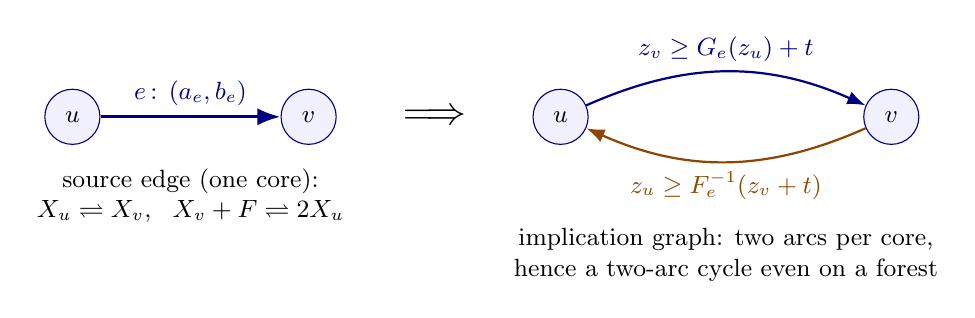
\begin{tikzpicture}[>=Latex,
  sp/.style={circle,draw=blue!50!black,fill=blue!6,minimum size=7mm,inner sep=0pt,font=\small}]
\node[sp] (u) at (0,0) {$u$};
\node[sp] (v) at (3.0,0) {$v$};
\draw[->,very thick,blue!50!black] (u)--(v) node[midway,above,font=\small] {$e$\,: $(a_e,b_e)$};
\node[font=\small,align=center] at (1.5,-1.0) {source edge (one core):\\ $X_u\rev X_v,\ \ X_v+F\rev 2X_u$};
\node[font=\Large] at (4.6,0) {$\Longrightarrow$};
\node[sp] (u2) at (6.2,0) {$u$};
\node[sp] (v2) at (10.4,0) {$v$};
\draw[->,thick,blue!50!black] (u2) to[bend left=24] node[midway,above,font=\small] {$z_v\ge G_e(z_u)+t$} (v2);
\draw[->,thick,orange!55!black] (v2) to[bend left=24] node[midway,below,font=\small] {$z_u\ge F_e^{-1}(z_v+t)$} (u2);
\node[font=\small,align=center] at (8.3,-1.75) {implication graph: two arcs per core,\\ hence a two-arc cycle even on a forest};
\end{tikzpicture}
\caption{Three kinds of cycle must be kept apart. \emph{Directed source cycles} are never compatible. \emph{Undirected source cycles} with acyclic orientation may be compatible and are allowed. \emph{Implication cycles} live in the bidirected graph used by the algorithms and exist for every instance with at least one core.}
\label{fig:implications}
\end{figure}

The \emph{implication graph} has vertex set $V$ and both arcs $u\to v$ and $v\to u$ for every source edge (Figure~\ref{fig:implications}); it has $2|E|$ arcs. A \emph{simple implication path} $\pi$ from $s$ to $v$ visits no vertex twice; the path of length zero is included, with the identity as its map; $f_{\pi,t}$ denotes the composition of the implication maps along $\pi$. A \emph{rooted simple implication cycle} $c$ at $j$ returns to $j$ and repeats no other vertex; the two-arc cycles $u\to v\to u$ are included; $T_{c,t}$ is its composite map. The subscript $t$ is dropped when the margin is fixed. Because the source graph is simple, an implication cycle with at least three arcs is a simple cycle of the underlying graph, so
\begin{equation}\label{eq:lengths}
  \text{a simple path has at most } h \text{ arcs, and a rooted simple cycle at most } h+1 .
\end{equation}

\begin{lemma}[Min-closure and least state]\label{lem:least}
For every $t\ge0$ the set $\St$ is compact and closed under coordinatewise minimum. If it is nonempty it has a least element $z_*(t)$, and every coordinate of $z_*(t)$ either equals $\ell_v$ or is tight in some incoming implication, $z_*(t)_v=f(z_*(t)_i)$.
\end{lemma}
\begin{proof}
Compactness is clear. Let $z,z'\in\St$ and $w=\min(z,z')$, and consider an implication $z_j\ge f(z_i)$ with $f$ increasing. If $w_j=z_j$ then $w_j=z_j\ge f(z_i)\ge f(w_i)$, and symmetrically otherwise. Boxes are preserved. A compact min-closed set has a least element: a minimizer of $\sum_v z_v$ must lie below every other element, since otherwise the minimum with that element would have a smaller sum. If a coordinate of $z_*$ were above $\ell_v$ and above all incoming implication values, lowering it to the maximum of those would preserve all constraints, as outgoing implications only become easier.
\end{proof}

\section{The least state at a fixed margin by exact cycle acceleration}\label{sec:acceleration}

Fix $t\ge0$. The statements of this section hold for real $t$. The algorithm maintains a vector of \emph{anchors} $A\in\R^V$, initially $A_v=\ell_v$, and a vector $D\ge A$ of \emph{labels}: each $D_v$ is stored as a vertex $s$ together with a simple implication path $\pi$ from $s$ to $v$, and has the value $f_\pi(A_s)$.

\medskip
\noindent\textbf{Algorithm 1} (fixed-margin closure by label correcting with cycle detection).
\begin{enumerate}[label=\arabic*.]
\item \emph{Start a phase.} Set $D_v\leftarrow A_v$ with the path of length zero, for every $v$.
\item \emph{One round.} If $D_v>u_v$ for some $v$, return \INF. Scan all implication arcs $e\colon i\to j$ using the values of $D$ at the beginning of the round. If $f_e(D_i)>D_j$, the arc is \emph{violated}; then
 \begin{enumerate}[label=(\alph*)]
 \item if $j$ lies on the path of the label $D_i$, a cycle is \emph{detected}: let $c$ be the rooted simple cycle at $j$ formed by the part of that path from $j$ to $i$ followed by $e$, and go to step~3;
 \item otherwise the path of $D_i$ extended by $e$ is a candidate label for $j$.
 \end{enumerate}
 If no arc is violated, return $D$. Otherwise give every $j$ with candidates the candidate of largest value and start the next round.
\item \emph{Jump.} Let $\alpha$ be the least solution of $T_c(\alpha)=\alpha$ in $(D_j,u_j]$. If there is none, return \INF. Otherwise set $A_j\leftarrow\alpha$, leave all other anchors unchanged, and go to step~1.
\end{enumerate}

\noindent Three design decisions matter. Labels are only ever extended to simple paths, so no path enumeration is needed and a phase is short (Lemma~\ref{lem:rounds}). The jump target is the least fixed point \emph{strictly above the current value} $D_j$, which need not be the least fixed point of $T_c$. And $D$ is recomputed from the anchors in every phase but never installed as the new anchor vector, so that an anchor is always an original lower endpoint or a root of one fixed cycle map, whose coefficients do not depend on the state of the computation.

\begin{lemma}[Short phases]\label{lem:rounds}
All labels are simple paths from anchors. A label created in round $r$ of a phase has at least $r$ arcs. Consequently a phase has at most $h+1$ rounds, each of which scans the $2|E|\le2hn$ arcs once.
\end{lemma}
\begin{proof}
Step 2(b) extends a simple path by an arc to a vertex not on it. A label created in round one has one arc. Suppose the arc $e\colon i\to j$ is violated in round $r+1\ge2$. If the label $D_i$ had not been created in round $r$, its value was the same at the beginning of round $r$, when the arc was scanned. Either it was not violated then, and $D_j\ge f_e(D_i)$ has held ever since because labels only increase; or it was violated, no cycle was detected since the phase continued, and $D_j$ received a candidate of value at least $f_e(D_i)$. Both contradict the violation in round $r+1$. Hence $D_i$ was created in round $r$ and has at least $r$ arcs by induction, and a label created from it in round $r+1$ has at least $r+1$. By \eqref{eq:lengths} a simple path has at most $h$ arcs, so every violated arc in round $h+1$ leads to a detection. The bound on $|E|$ is Proposition~\ref{prop:graphs}(a).
\end{proof}

\begin{lemma}[Forced cycle root]\label{lem:jump}
Assume every element of $\St$ dominates $A$. Then every element of $\St$ dominates $D$ throughout the phase. At a detection, $T_c(D_j)>D_j$. If $\St\ne\varnothing$, step~3 finds a root $\alpha$, and every element of $\St$ dominates the updated anchors.
\end{lemma}
\begin{proof}
Let $z\in\St$. Along a path $\pi\colon s\leadsto v$, monotonicity and the implications satisfied by $z$ give $f_\pi(A_s)\le f_\pi(z_s)\le z_v$, hence $D\le z$. At a detection, the part of the path of $D_i$ that ends at $j$ was the label of $j$ in an earlier round of the phase; its value $a$ satisfies $a\le D_j$ because labels only increase within a phase. By construction $T_c(a)=f_e(D_i)>D_j\ge a$, and monotonicity of $T_c$ gives $T_c(D_j)\ge T_c(a)>D_j$. Now let $z\in\St$. Going around $c$ gives $T_c(z_j)\le z_j$, and $D_j\le z_j\le u_j$. The continuous function $T_c(x)-x$ is positive at $D_j$ and nonpositive at $z_j$, so it vanishes somewhere in $(D_j,z_j]$. Its zero set in $[D_j,u_j]$ is closed and does not contain $D_j$, so it has a least element $\alpha>D_j$, and $\alpha\le z_j$. Since $z$ was arbitrary, the updated anchor vector is dominated by all of $\St$.
\end{proof}

\begin{lemma}[Finite progress and correctness]\label{lem:termination}
Algorithm~1 terminates. It returns \INF{} if and only if $\St=\varnothing$, and otherwise returns the least element $z_*(t)$ of $\St$. The number $J$ of jumps is at most the number of pairs $(c,\alpha)$ with $c$ a rooted simple cycle whose map is not the identity and $\alpha\in[0,u_j]$ a fixed point of $T_c$.
\end{lemma}
\begin{proof}
Each $T_c$ is real analytic on a connected neighbourhood of $[0,u_j]$. By the identity theorem \citep{krantz2002}, either $T_c$ is the identity there or $T_c(x)-x$ has finitely many zeros in the compact interval. A detected cycle has $T_c(D_j)>D_j$ and is not of the first kind. There are finitely many rooted simple cycles, so the set of pairs $(c,\alpha)$ in the statement is finite. A jump with token $(c,\alpha)$ sets $A_j=\alpha>D_j\ge A_j^{\mathrm{old}}$, and anchors never decrease, so afterwards $D_j\ge A_j\ge\alpha$ forever. A later jump on the same rooted cycle selects a root strictly above the then current $D_j\ge\alpha$. Hence no token is used twice, and by Lemma~\ref{lem:rounds} the algorithm stops.

By Lemma~\ref{lem:jump} the invariant ``$\St$ dominates $A$'' holds throughout. An overflow exit contradicts $D\le z\le u$ for $z\in\St$, and an exit in step~3 contradicts the existence of a root; so both occur only when $\St=\varnothing$. When no arc is violated, $D$ lies in the boxes, because $\ell\le A\le D\le u$, and satisfies all implications, so $D\in\St$; being dominated by every element of $\St$, it is the least one.
\end{proof}

Margin zero is included: at $t=0$ some cycle maps can be identities, with a continuum of fixed points (Remark~\ref{rem:failures}), but such a cycle is never detected, because detection exhibits a strict violation.

\begin{corollary}[Bounded ancestry]\label{cor:ancestry}
Every value that Algorithm~1 computes, and in particular each coordinate of its output, has the form $f_\pi(\sigma)$, where $\pi$ is a simple implication path from a vertex $s$ and the \emph{seed} $\sigma$ is either $\ell_s$ or a fixed point in $(\ell_s,u_s]$ of the map of one rooted simple cycle at $s$. By \eqref{eq:lengths} such a description involves at most $2h+1$ implication maps, independently of the number of jumps.
\end{corollary}

\begin{example}[One unit core]\label{ex:unitedge}
Take one edge $u\to v$ with $a=b=1$, boxes $[\tfrac1{10},\tfrac9{10}]$ and $[\tfrac1{100},\tfrac9{10}]$, and $t=\tfrac1{100}$. Here $G(x)=(x+2x^2)/3$ and $F^{-1}(y)=(-1+\sqrt{1+8y})/2$. In round one only the arc $u\to v$ is violated, and $D$ becomes $(\tfrac1{10},\tfrac1{20})$ with $D_v=G(\tfrac1{10})+t$ labelled by the path $u\to v$. In round two the arc $v\to u$ is violated, since $F^{-1}(\tfrac1{20}+t)\approx0.1083>D_u$, and $u$ lies on the path of $D_v$: the two-arc cycle at $u$ with map $T_c=F^{-1}\circ(G+2t)$ is detected. Its fixed points solve $F(x)-G(x)=2t$, that is $x(1-x)=12t$, so the least root above $D_u$ is $\alpha=(5-\sqrt{13})/10\approx0.1394$. In the next phase $D=(\alpha,\alpha-\tfrac7{100})$ satisfies both implications with equality, and the algorithm returns it: the least state is irrational, and it was reached in one jump. Iterating $T_c$ from $D_u$ instead converges to $\alpha$ linearly and never reaches it (Figure~\ref{fig:cycle}). In the margin, the two roots of $x(1-x)=12t$ merge at $t=\tfrac1{48}$, beyond which $\St=\varnothing$.
\end{example}

\begin{figure}[t]
\centering
\includegraphics[width=\linewidth]{figures/cycle.pdf}
\caption{Example~\ref{ex:unitedge}. (a) The detected cycle map lies above the diagonal at the current value, which forces every feasible seed above the next fixed point $\alpha$. (b) Plain iteration of the same map approaches $\alpha$ geometrically without terminating. (c) The two root branches of the cycle as functions of the margin; they are ordered and continuous for small $t$ and merge in a double root at $t=1/48$. All curves are exact formulas.}
\label{fig:cycle}
\end{figure}

\begin{remark}[Why simpler schemes fail]\label{rem:failures}
Three exact examples shaped the algorithm; each is replayed by the script of Appendix~\ref{app:repro}.

(a) \emph{Policies.} A tempting scheme selects, for each coordinate, one incoming implication that is tight at the least state (Lemma~\ref{lem:least}), and solves the selected equalities. Take unit cores $x\to y$ and $x\to z$, margin $t=\tfrac1{64}$, and boxes $x\in[\tfrac18,\tfrac78]$, $y\in[\tfrac1{16},\tfrac78]$, $z\in\{\tfrac{41}{64}\}$. The least state is $(\tfrac34,\tfrac{41}{64},\tfrac{41}{64})$. The policy that uses the two implications of the core $x\to y$ is tight there, but its own least solution is $(\tfrac14,\tfrac9{64},\tfrac{41}{64})$, which violates the omitted constraint $z+t\le F(x)$ by exactly $\tfrac12$. These statements are compiled (module \lean{Interaction}). A six-species instance in the repository shows that the same failure occurs when the tight policy is unique. This is why Algorithm~1 never solves a selected subsystem: it only installs lower bounds that are forced on every feasible state, and it keeps every original inequality in the final test.

(b) \emph{Identity cycles at margin zero.} Put unit ratios on a two-core path and ratio $2$ on a parallel two-core path with the same endpoints. Since $G_2=F_1=:F$, the upper response of the first path equals the lower response of the second, and at $t=0$ the corresponding implication cycle is the identity, with a continuum of fixed points. For every $t>0$ the two paths are contradictory, since $F(F(x)-t)-t-\bigl(F(F(x)+t)+t\bigr)=-t(x^2+x+3)<0$. Positive margins therefore separate finite root sets from identity continua.

(c) \emph{Intervals and binary search.} On forests, feasible projections are intervals. With undirected cycles, two paths between the same species give responses whose order can switch several times, so the projection of the feasible set to one species is a disconnected union of intervals. Interval messages are then unsound, and so is the binary search on a variable that underlies the linear two-variable theory. Section~\ref{sec:fpt} represents such projections exactly by next-maps.
\end{remark}

\section{Labels and branch-preserving elimination}\label{sec:elimination}

Algorithm~1 decides $\St\neq\varnothing$ for a given $t$. By \eqref{eq:strictiff} strict compatibility asks about all small positive $t$, and running the algorithm at $t=1,\tfrac12,\tfrac14,\dots$ never certifies that none works. This section shows that every comparison the algorithm makes has a constant outcome for small positive $t$, with an explicit meaning of ``small''.

\subsection{Labels and local tests}
A \emph{seed specification} at a vertex $s$ is either the constant $\ell_s$, or a rooted simple cycle $c$ at $s$; in the second case the admissible seeds at margin $t$ are the elements of
\[
  \mathrm{Fix}_c(t)=\{\sigma\in[0,u_s]\;:\;T_{c,t}(\sigma)=\sigma\}.
\]
A \emph{label template} $\lambda$ at $v$ is a seed specification at some $s$ together with a simple implication path $\pi$ from $s$ to $v$; its value is $\val_\lambda(t,\sigma)=f_{\pi,t}(\sigma)$, where $\sigma$ is the seed. Intermediate values of a transport are nonnegative but are not required to lie in the species boxes: a path may overshoot, and the box tests detect it.

\begin{lemma}[Finite fibres]\label{lem:fibres}
For $t>0$ no cycle map is the identity, and every $\mathrm{Fix}_c(t)$ is finite.
\end{lemma}
\begin{proof}
For $t>0$ every implication map is positive at $0$ and increasing, so $T_{c,t}(0)>0$. Analyticity on a neighbourhood of $[0,u_s]$ and the identity theorem give finiteness.
\end{proof}

A \emph{local test} is one of the following statements about actual label values:
\begin{itemize}
\item[(B)] a box test $\ell_v\le\val_\lambda$ or $\val_\lambda\le u_v$ for a label at $v$;
\item[(E)] an edge test $G_e(\val_\lambda)+t\le\val_\mu$ or $\val_\mu+t\le F_e(\val_\lambda)$ for an edge $e\colon u\to v$, a label $\lambda$ at $u$ and a label $\mu$ at $v$;
\item[(O)] an order test $\val_\lambda\le\val_\mu$ or $\val_\lambda<\val_\mu$ for two labels at the same vertex, which includes the comparison of a cycle root (a label with a path of length zero) with another label.
\end{itemize}
By Corollary~\ref{cor:ancestry} these are all the comparisons of Algorithm~1: the violation test of an arc is of type (E), the choice of the largest candidate and the selection of the least root above $D_j$ are of type (O), and the overflow and root-range tests are of type (B). Each test involves at most two seeds.

\subsection{Quadratic descriptions and projection with the seeds kept free}
With $a=a_1/a_2$, $b=b_1/b_2$ in lowest terms, a forward step $y=G_{a,b}(x)+t$ and a reverse step $y=F_{a,b}^{-1}(x+t)$ are described by
\begin{align}
 (a+2b)y-ax-2bx^2-(a+2b)t&=0,\qquad x,y\ge0,\label{eq:forwardgraph}\\
 ay+by^2-(a+b)x-(a+b)t&=0,\qquad x,y\ge0,\label{eq:reversegraph}
\end{align}
which after multiplication by $a_2b_2$ are integer polynomials of degree two with coefficients of at most $2B+2$ bits. The sign condition $y\ge0$ in \eqref{eq:reversegraph} is essential: $ay+by^2$ is strictly increasing from $0$ to $\infty$ on $y\ge0$, so for nonnegative $x$ and $t$ there is exactly one admissible $y$.

\begin{lemma}[Projection with fixed seeds]\label{lem:projection}
Let $\Theta$ be a local test, or the membership statement $\sigma\in\mathrm{Fix}_c(t)$. There is a quantifier-free formula $\Theta^{\mathrm{qf}}$ in $t$ and the at most two seed variables such that, for all $t\ge0$ and all nonnegative seed values, $\Theta^{\mathrm{qf}}$ holds if and only if $\Theta$ holds for the labels transported from \emph{those} seeds. It is obtained by eliminating one block of at most $4h+6$ existentially quantified variables from a conjunction of at most $8h+16$ polynomial equations and weak or strict inequalities of degree at most two.
\end{lemma}
\begin{proof}
Introduce one variable for the output of every step of the cycles and paths involved, state \eqref{eq:forwardgraph} or \eqref{eq:reversegraph} for every step, and add the final comparison, or for membership the equation ``last value $=\sigma$'' and the bounds $0\le\sigma\le u_s$. By \eqref{eq:lengths} two cycles and two paths have at most $4h+2$ steps, and a test of type (E) adds one more quadratic inequality. Once $t$ and the seeds are fixed, every step has exactly one admissible output, so by induction there is exactly one admissible tuple of internal values, namely the actual transport. The existential closure over the internal variables is therefore equivalent to the statement about the actual labels. In particular it does \emph{not} replace the given seed by some other root of the same cycle, because the seed is not quantified. Real quantifier elimination \citep{tarski1951,bpr2006} provides $\Theta^{\mathrm{qf}}$.
\end{proof}

Eliminating the seeds as well would answer the question whether \emph{some} root passes a test. That is not the question Algorithm~1 asks, and it would lose the identity of the branch; the six-species instance of Remark~\ref{rem:failures}(a) shows that the wrong root can pass a test that the right root fails.

\subsection{Ordered branches for small margins}
For a local test $\Theta$ with seed variables among $(\sigma,\sigma')$, let $\mathcal{P}_\Theta\subset\Z[t,\sigma,\sigma']$ consist of $t$, the polynomials of $\Theta^{\mathrm{qf}}$, and the polynomials of the membership formulas of the cycles involved. Fix a cylindrical algebraic decomposition (CAD) of $\R^3$, $\R^2$ or $\R$ adapted to $\mathcal{P}_\Theta$, with variable order $t,\sigma,\sigma'$ \citep{collins1975,bpr2006}: a partition into finitely many connected cells, arranged in stacks of sections (graphs of continuous functions) and sectors (bands between them) over the cells of the decomposition induced on the first coordinates, such that every polynomial of $\mathcal{P}_\Theta$ has constant sign on every cell. We use complete decompositions, with all cells of lower dimension; no genericity, squarefreeness or well-orientedness is assumed. Do the same for the membership formula of each cycle involved, alone, in the variables $(t,\sigma)$. Let $\mathcal{U}_\Theta$ be the finite list of all nonzero univariate polynomials in $t$ that define the base decompositions of these CADs, divided by the largest power of $t$ that divides them, and let $H_\Theta\ge1$ bound the binary lengths of their integer coefficients. A polynomial $\sum_{i\le m}c_it^i$ with integer coefficients and $c_0\ne0$ has no complex root of modulus less than $|c_0|/(|c_0|+\max_{i\ge1}|c_i|)$, by Cauchy's bound applied to the reciprocal polynomial \citep{mignotte1992}; this is more than $1/(1+2^{H_\Theta})\ge2^{-(H_\Theta+1)}$. Hence the interval
\begin{equation}\label{eq:dtheta}
   I_\Theta=(0,d_\Theta),\qquad d_\Theta=2^{-(H_\Theta+1)},
\end{equation}
contains no root of any member of $\mathcal{U}_\Theta$ and lies in one open base cell of every decomposition attached to $\Theta$.

\begin{lemma}[Consistent ordered branches]\label{lem:branches}
Let $\Theta$ be a local test.
\begin{enumerate}[label=(\alph*)]
\item For every cycle $c$ involved in $\Theta$ there are an integer $m_c\ge0$ and continuous functions $\rho_{c,1}<\dots<\rho_{c,m_c}$ on $I_\Theta$ such that $\mathrm{Fix}_c(t)=\{\rho_{c,1}(t),\dots,\rho_{c,m_c}(t)\}$ for every $t\in I_\Theta$. Here $\rho_{c,i}(t)$ is the $i$-th smallest element of $\mathrm{Fix}_c(t)$, so the indexing does not depend on the decomposition or on $\Theta$.
\item For every choice of branch indices for its seeds, the truth value of $\Theta$ at the seeds $\rho_{c,i}(t)$, $\rho_{c',i'}(t)$ is the same for all $t\in I_\Theta$.
\end{enumerate}
\end{lemma}
\begin{proof}
(a) A polynomial in $(t,\sigma)$ has constant sign on every cell of the decomposition of the $(t,\sigma)$-plane, so the membership formula has a constant truth value on each cell over $I_\Theta$. A sector on which it held would make $\mathrm{Fix}_c(t)$ infinite, contradicting Lemma~\ref{lem:fibres}. Hence the set $\{(t,\sigma):t\in I_\Theta,\ \sigma\in\mathrm{Fix}_c(t)\}$ is a union of sections over $I_\Theta$, which are graphs of continuous functions that do not meet; ordering them gives the $\rho_{c,i}$.

(b) Consider a test with two seeds and its CAD of $\R^3$; the cases with fewer seeds are simpler. Every cell of $\R^3$ over a cell $C$ of the induced decomposition of the $(t,\sigma)$-plane projects onto all of $C$, so a polynomial of $\mathcal{P}_\Theta$ that does not involve $\sigma'$ has constant sign on $C$. Thus the induced decomposition is adapted to the membership polynomials of $c$, and the graph $C_i$ of $\rho_{c,i}$ over $I_\Theta$ is one of its sections: a section over $I_\Theta$ on which membership holds is the graph of a continuous function with values in $\{\rho_{c,1}(t),\dots,\rho_{c,m_c}(t)\}$, hence one of the $\rho_{c,i}$ by connectedness. In the stack over $C_i$, the membership formula of $c'$ is constant on each cell and has finite fibres, so it holds only on sections. Such a section is the graph of a continuous function $\zeta$ on the connected set $C_i$ with $\zeta(t,\sigma)\in\{\rho_{c',1}(t),\dots,\rho_{c',m_{c'}}(t)\}$; since the $\rho_{c',i'}$ are continuous and strictly ordered on $I_\Theta$, the index is locally constant, hence constant. Consequently the curve $t\mapsto(t,\rho_{c,i}(t),\rho_{c',i'}(t))$, $t\in I_\Theta$, stays inside a single cell of $\R^3$. The formula $\Theta^{\mathrm{qf}}$ has a constant truth value on that cell, and by Lemma~\ref{lem:projection} this is the truth value of $\Theta$ on the actual labels.
\end{proof}

\section{The margin as a positive infinitesimal, and rational output}\label{sec:threshold}

\noindent\textbf{Algorithm 2} (strict decision). If $E=\varnothing$, return $\ell$. Otherwise run Algorithm~1 \emph{symbolically at $t=0^+$}: an anchor is stored as the constant $\ell_s$ or as a pair (rooted simple cycle, branch index), a label as an anchor with a simple path, and every local test $\Theta$ is answered by its constant truth value on $I_\Theta$ from Lemma~\ref{lem:branches}; in step~3 the branches of $c$ are enumerated in increasing order and the first one that passes the tests $D_j<\rho_{c,i}$ and $\rho_{c,i}\le u_j$ is selected. Let $\Theta_1,\dots,\Theta_N$ be the tests performed and put
\begin{equation}\label{eq:threshold}
  H=\max_k H_{\Theta_k},\qquad t_1=2^{-(H+2)} .
\end{equation}
If the symbolic run returns \INF, report that no productive state exists. Otherwise evaluate the returned labels at the margin $t_1$ and return the rounding of Lemma~\ref{lem:round}.

\begin{theorem}[Trace invariance]\label{thm:trace}
The symbolic run terminates after at most $\sum_cm_c$ jumps. For every real $t\in(0,2^{-(H+1)})$, Algorithm~1 at margin $t$, with the same scanning order, performs the same sequence of tests with the same outcomes, where the branch index $i$ of a cycle $c$ stands for the root $\rho_{c,i}(t)$. Consequently, if the symbolic run returns \INF{} then $\St=\varnothing$ for all $t>0$ and no productive state exists; otherwise its labels evaluated at $t$ form the least element of $\St$ for every $t\in(0,2^{-(H+1)})$, and a productive state exists.
\end{theorem}
\begin{proof}
Let $t\in(0,2^{-(H+1)})$, so that $t\in I_{\Theta_k}$ for every $k$. By induction on the number of tests, the real run at $t$ and the symbolic run are in corresponding states: same anchors and labels under the correspondence $i\mapsto\rho_{c,i}(t)$, which is a bijection onto $\mathrm{Fix}_c(t)$ preserving order. The next test is therefore the same local test, and by Lemma~\ref{lem:branches}(b) its real outcome at $t$ is the symbolic outcome. In step~3 the real algorithm selects the least root of $T_c$ in $(D_j,u_j]$, which is the first branch passing the two tests. For the termination of the symbolic run, apply the same argument to each finite initial segment of it, whose tests define some $H'$: the real run at any $t<2^{-(H'+1)}$ agrees with that segment, real runs never reuse a token $(c,\alpha)$ by Lemma~\ref{lem:termination}, and tokens correspond to pairs $(c,i)$. So no pair $(c,i)$ is used twice in the symbolic run. The conclusions follow from Lemma~\ref{lem:termination} at each such $t$, together with the monotonicity of $\St$ in $t$ and \eqref{eq:strictiff}.
\end{proof}

Only the tests that are actually performed are ever decomposed, and the threshold $t_1$ is as large as those tests allow. A zero optimal margin, as in Remark~\ref{rem:failures}(b), is rejected by one terminating run.

\begin{lemma}[Downward rational reconstruction]\label{lem:round}
Let $t>0$, $z\in\St$, and let $N$ be a power of two with $1/N\le t/4$. The vector
\[
   q_v=\max\bigl\{\ell_v,\ \lfloor Nz_v\rfloor/N\bigr\}
\]
is rational, lies in the boxes, and belongs to $\Sset{t/2}$; in particular it is productive. Singleton boxes are reproduced exactly. Each $q_v$ is found with $O(\log N)$ comparisons of $z_v$ with dyadic rationals.
\end{lemma}
\begin{proof}
Put $\eta=1/N$. By construction $\ell_v\le q_v\le z_v\le u_v$ and $z_v-q_v<\eta$. Since rounding is downward and $G_e$ is increasing, $q_v-G_e(q_u)\ge z_v-\eta-G_e(z_u)\ge t-\eta$. Since $0<F_e'\le2$ on $[0,1]$, $F_e(q_u)-q_v\ge F_e(z_u)-2\eta-z_v\ge t-2\eta\ge t/2$. The integer $\lfloor Nz_v\rfloor\in[0,N]$ is located by bisection, each step being a comparison of $z_v$ with a dyadic rational. One rounded value is used for every occurrence of a species.
\end{proof}

The one-sided estimate, compiled as \lean{round_down_margin}, loses $2\eta$ where a two-sided perturbation would lose $3\eta$. It shows that an algebraic state of margin $t>\mu\ge0$ rounds to a rational state of margin at least $\mu$ as soon as $\eta\le(t-\mu)/2$. It does not give a rational state at a prescribed \emph{weak} margin: the least state at margin $t$ can be irrational (Example~\ref{ex:unitedge}).

\begin{corollary}[A uniform threshold]\label{cor:uniform}
Let $H_{\max}$ be the maximum of $H_\Theta$ over \emph{all} local tests of the instance and $t_0=2^{-(H_{\max}+2)}$. Then a productive state exists if and only if $\Sset{t_0}\neq\varnothing$, and $\St\ne\varnothing$ either for all or for no $t\in(0,2t_0)$.
\end{corollary}
\begin{proof}
Let $t,t'\in(0,2t_0)$ and $\St\neq\varnothing$. By Corollary~\ref{cor:ancestry} and Lemma~\ref{lem:termination}, each coordinate of $z_*(t)$ is the value of a label template at a seed $\rho_{c,i}(t)$ or $\ell_s$. The vector of the same templates and indices at $t'$ passes all tests (B) and (E) that express membership in $\Sset{t'}$, by Lemma~\ref{lem:branches}(b). The rest is \eqref{eq:strictiff}.
\end{proof}

An independent proof of the completeness of labels avoids the algorithm: by Lemma~\ref{lem:least} each coordinate of the least state not at its lower endpoint has a tight incoming implication, and following tight predecessors either reaches a lower endpoint or closes a rooted simple cycle of which the value is a fixed point. The corollary is the form in which the Lean root theorem of Section~\ref{sec:formal} is stated. Algorithm~2 does not compute $t_0$, which would require all $(n+2)^{O(h)}$ templates.

\section{Bit complexity of cycle acceleration}\label{sec:complexity}

A cylindrical decomposition in all $n$ variables would be doubly exponential in $n$ \citep{davenport1988}. The analysis rests on two facts from Section~\ref{sec:elimination}: the variables eliminated in a block are uniquely determined, so that the block costs singly exponentially in its length $O(h+1)$, and the decompositions live in at most three variables.

We use the following published bounds. (QE) For $s$ polynomials of degree at most $d$ in $m+\ell$ variables with integer coefficients of at most $\tau$ bits, one block of $m$ existential quantifiers is eliminated with $s^{(m+1)(\ell+1)}d^{O(m)O(\ell)}$ arithmetic operations; the output has at most that many polynomials, of degree $d^{O(m)}$, and all integers in the computation and the output have at most $\tau d^{O(m)O(\ell)}$ bits \citep[Theorem 2.27]{basu2014}, \citep[Chapter 14]{bpr2006}. (CAD) For a fixed number of variables, a complete cylindrical decomposition adapted to $S$ integer polynomials of degree at most $D$ and coefficient length at most $L$, with sample points and the signs of the polynomials on all cells, is computed with a number of bit operations polynomial in $S$, $D$ and $L$ \citep{collins1975}, \citep[Chapter 11]{bpr2006}. (RI) The real roots of an integer polynomial are isolated, and compared with rationals and with each other, in bit time polynomial in its degree and coefficient length \citep{sagraloff2016,bpr2006}.

\begin{lemma}[Local arithmetic]\label{lem:bits}
Put $k=h+1$. There are absolute constants $C_0,c_0$ such that, with $Q=(k+1)^{C_0k}$:
\begin{enumerate}[label=(\alph*)]
\item every formula $\Theta^{\mathrm{qf}}$ of Lemma~\ref{lem:projection} has at most $Q$ polynomials, of degree at most $Q$ and coefficient length at most $(B+1)Q$, and is computed in at most $Q(B+1)^{c_0}$ bit operations;
\item the same bounds hold for the decompositions attached to $\Theta$, so that $H_\Theta\le(B+1)Q$, every cycle has $m_c\le Q$ branches, and the outcome of $\Theta$ on $I_\Theta$ for given branch indices is found within $Q(B+1)^{c_0}$ bit operations;
\item for a rational $t$ of $O((B+1)Q)$ bits, each local test at given branch indices, and each comparison of a label at given branch index with a rational of $O((B+1)Q)$ bits, is decided in at most $Q(B+1)^{c_0}$ bit operations.
\end{enumerate}
\end{lemma}
\begin{proof}
(a) Apply (QE) with $m\le4h+6$, $s\le8h+16$, $d=2$, $\ell\le3$ and $\tau\le2B+2$. The operation count is $(8k+8)^{4(4k+3)}2^{O(k)}=(k+1)^{O(k)}$, degrees are $2^{O(k)}$, and integers have $(2B+2)2^{O(k)}$ bits. Multiplying the operation count by the cost of one arithmetic operation on such integers gives the bit cost.

(b) Apply (CAD) in at most three variables to the at most $3Q+1$ polynomials of $\mathcal{P}_\Theta$. The cost and the sizes of all projection polynomials, in particular of the members of $\mathcal{U}_\Theta$, are polynomial in $Q$ and $(B+1)Q$; enlarging $C_0$ and $c_0$ restores the stated form. The members of $\mathcal{U}_\Theta$ are kept as a list and are not multiplied together. A finite set defined by a quantifier-free formula in one variable consists of roots of its polynomials, which bounds $m_c$. The cell of the curve of Lemma~\ref{lem:branches}(b) is identified from the sample point of the base cell $I_\Theta$ by counting sections in the two stacks.

(c) Substituting a rational $t$ into a polynomial of degree at most $Q$ and clearing denominators adds $O(Q\cdot(B+1)Q)$ bits to each coefficient, which is again absorbed. Membership becomes a univariate formula: isolate the roots of its polynomials by (RI), keep those at which the formula holds, and number them increasingly. A test with two seeds becomes a formula in $(\sigma,\sigma')$, evaluated at the pair of indexed roots by a decomposition of the plane, or equivalently by sign determination at a pair of real algebraic numbers \citep[Chapters 10--11]{bpr2006}. A rational constant in a comparison is absorbed in the same way.
\end{proof}

\begin{proof}[Proof of Theorem~\ref{thm:main}]
Correctness is Theorem~\ref{thm:trace} and Lemma~\ref{lem:round}. Let $E\ne\varnothing$. By Lemma~\ref{lem:rounds} a phase consists of at most $h+1$ rounds of at most $2hn$ arc scans, each of which is one test (E), one membership lookup in a stored path, and at most one test (O) per candidate, plus $n$ overflow tests (B) per round. A jump enumerates at most $Q$ branches with two tests each. So a phase costs $O(h^2n+Q)$ local tests, each within $Q(B+1)^{c_0}$ bit operations by Lemma~\ref{lem:bits}(b); indices and stored paths have $O(h\log(n+2))$ bits. There are $J+1$ phases. No number field generated by earlier roots is ever constructed: by Corollary~\ref{cor:ancestry} every comparison is between two labels of bounded description.

For the output, $t_1$ has $H+2\le(B+1)Q+2$ bits, and Lemma~\ref{lem:round} with $\log N=H+4$ uses $O(H)$ comparisons per species of a label at the rational margin $t_1$ with a dyadic rational of $O(H)$ bits, each covered by Lemma~\ref{lem:bits}(c); the output has $O(n(B+H))$ bits. Altogether the cost is $(J+1)\,n\,Q^{O(1)}(B+\log(n+2)+1)^{O(1)}$, which is \eqref{eq:mainbound}.

By Theorem~\ref{thm:trace}, $J\le\sum_cm_c\le\sigma Q$. A rooted simple cycle is either one of the $2|E|\le2hn$ two-arc cycles (counted with their root) or a sequence of at most $h+1$ distinct vertices, which gives $\sigma\le2hn+(n+1)^{h+1}$; and $Q\le(n+2)^{O(h)}$ because $h+1\le n$. If the underlying graph has $O(n)$ simple cycles of length at least three, counted with their $2(h+1)$ rootings and directions, then $\sigma=O(hn)$.
\end{proof}

On a forest the only implication cycles are the two-arc cycles, whose fixed-point equation $F_e(x)-G_e(x)=2t$ is quadratic, so $J\le4|E|$ and the cost is $n^2(h+2)^{O(h)}\poly(B)$. On a windmill $W_k$ (Section~\ref{sec:parameter}) there are $6k$ rooted two-arc cycles and $6k$ rooted directed triangles. On the complete bipartite graph $K_{q,n}$, by contrast, $h=2q$ and $\sigma=n^{\Theta(q)}$; whether $J$ can actually be that large is open (Section~\ref{sec:discussion}), and Theorem~\ref{thm:fpt} covers such families by a different algorithm.

The bound is a guarantee for the algorithm as specified, with complete projected decompositions as the exact fallback of every sign decision. An implementation that sends the $O(h)$ internal variables to a full-dimensional decomposition, or that merges the algebraic number fields of successive roots, is not covered by this analysis. We have not implemented the complete algorithm, and we make no claim about running times.

\section{Fixed-parameter tractability by monotone elimination}\label{sec:fpt}

\subsection{Monotone systems and next-maps}
Fix a real margin $t>0$. Let $\M$ be the class of functions $f\colon[0,\infty]\to[0,\infty]$ that are nondecreasing, left-continuous on $[0,\infty)$, and satisfy $f(\infty)=\infty$. It contains the implication maps \eqref{eq:maps} and is closed under composition and under finite pointwise maxima. A \emph{monotone system} on a vertex set $W$ consists of boxes $[\ell_v,u_v]$, maps $M_{ij}\in\M$ for ordered pairs $i\ne j$ (absent maps are $0$), and self-maps $T_v\in\M$ (initially $0$). A state $z\in\prod_v[\ell_v,u_v]$ is feasible if $z_j\ge M_{ij}(z_i)$ for all pairs and $z_v\ge T_v(z_v)$ for all $v$. The original problem at margin $t$ is the monotone system with $M_{uv}=g_{e,t}$ and $M_{vu}=k_{e,t}$ for every edge $e\colon u\to v$. The proof of Lemma~\ref{lem:least} applies verbatim: the feasible set is compact and min-closed, since a constraint $z_j\ge f(z_i)$ with $f$ nondecreasing and left-continuous defines a closed min-closed set.

The \emph{admissible set} and the \emph{next-map} of a vertex $w$ are
\begin{equation}\label{eq:nextmap}
  U_w=\{x\in[\ell_w,u_w]\;:\;T_w(x)\le x\},\qquad \nu_w(a)=\min\bigl(U_w\cap[a,\infty)\bigr),
\end{equation}
with $\nu_w(a)=\infty$ if $U_w\cap[a,\infty)$ is empty.
The set $U_w$ is closed, because $T_w$ is nondecreasing and left-continuous, so the minimum exists. It is in general a disconnected union of intervals; on a single unit core it is the interval between the two roots of Figure~\ref{fig:cycle}(c) intersected with the box. The map $\nu_w$ is the identity on $U_w$, is constant on every gap of $U_w$, and belongs to $\M$: if $a_k\uparrow a$ then the nondecreasing values $\nu_w(a_k)\in U_w$ converge to a point of the closed set $U_w$ that is at least $a$ and at most $\nu_w(a)$.

\begin{lemma}[Vertex elimination]\label{lem:eliminate}
Let $w$ be a vertex of a monotone system on $W$. Define a system on $W\setminus\{w\}$ by
\begin{equation}\label{eq:eliminate}
\begin{aligned}
  M'_{ij}&=\max\bigl(M_{ij},\ M_{wj}\circ\nu_w\circ M_{iw}\bigr)\quad(i\ne j), &
  T'_{i}&=\max\bigl(T_i,\ M_{wi}\circ\nu_w\circ M_{iw}\bigr),\\
  \ell'_j&=\max\bigl(\ell_j,\ M_{wj}(\nu_w(\ell_w))\bigr), & u'_j&=u_j,
\end{aligned}
\end{equation}
where a composite is $\infty$ wherever $\nu_w$ is. A state $z'$ on $W\setminus\{w\}$ is feasible for the new system if and only if it extends to a feasible state of the old one, and the least value of $z_w$ among all extensions is
\begin{equation}\label{eq:backsub}
  z_w=\nu_w\Bigl(\max\bigl\{\ell_w,\ \max_iM_{iw}(z'_i)\bigr\}\Bigr).
\end{equation}
\end{lemma}
\begin{proof}
Fix $z'$ satisfying the old constraints that do not involve $w$, and let $a$ be the maximum of $\ell_w$ and of the numbers $M_{iw}(z'_i)$. A value $x$ extends $z'$ if and only if $x\in U_w$, $x\ge a$, and $M_{wj}(x)\le z'_j$ for all $j$. If such an $x$ exists then $\nu_w(a)\le x$ is finite and $M_{wj}(\nu_w(a))\le M_{wj}(x)\le z'_j$ by monotonicity; conversely, if $\nu_w(a)$ is finite and satisfies these inequalities, it is an extension, and it is the least one. Since $\nu_w$ and $M_{wj}$ are nondecreasing, they commute with the maximum defining $a$, so the condition ``$M_{wj}(\nu_w(a))\le z'_j$ for all $j$'' is the conjunction over all $i$ and $j$ of $z'_j\ge M_{wj}(\nu_w(M_{iw}(z'_i)))$ and of $z'_j\ge M_{wj}(\nu_w(\ell_w))$. For $i\ne j$ these are the new implications, for $i=j$ the new self-constraints, and the last ones the new lower endpoints; finiteness of $\nu_w(a)$ is implied because a composite is $\infty$ where $\nu_w$ is.
\end{proof}

This is the order-theoretic core of the algorithm, and it is compiled in Lean for arbitrary index types and arbitrary monotone maps (declarations \lean{IsNextMap}, \lean{eliminate_vertex_iff}, \lean{eliminated_value_least}; Section~\ref{sec:formal}). The self-constraint $z_i\ge T'_i(z_i)$ is where cycles of the graph go: eliminating $v$ from one unit core $u\to v$ gives $T'_u=k_{e,t}\circ\nu_v\circ g_{e,t}$, which on the box of $v$ is the cycle map of Example~\ref{ex:unitedge}. The upper endpoint $u_w$ needs no separate rule, because it is part of $U_w$ and an inadmissible lower bound produces the value $\infty$.

\medskip
\noindent\textbf{Algorithm 3} (elimination along a depth-first forest, at a fixed margin). Compute a depth-first forest of the underlying graph. Eliminate the vertices in post-order by Lemma~\ref{lem:eliminate}, storing $\nu_w$, the maps $M_{iw}$ and $\ell_w$ at the time $w$ is eliminated. For a root $r$ there is nothing to update; if $\nu_r(\ell_r)=\infty$ return \INF. Then assign values in reverse order: $z_r=\nu_r(\ell_r)$ for roots, and \eqref{eq:backsub} with the stored data for the other vertices.

\begin{proposition}[Correctness]\label{prop:elimcorrect}
In a depth-first forest every edge joins a vertex to one of its ancestors. Hence, when $w$ is eliminated, all nonzero maps $M_{iw},M_{wj}$ join $w$ to its ancestors, every generated map joins two ancestors of $w$, and a vertex has at most $h$ ancestors. Algorithm~3 returns \INF{} if and only if $\St=\varnothing$, and otherwise returns the least element of $\St$.
\end{proposition}
\begin{proof}
The structural claims follow by induction from \eqref{eq:eliminate}. By Lemma~\ref{lem:eliminate} the system after each elimination is the exact projection of the previous one. After all non-root vertices of a tree have been eliminated, the root is feasible exactly on $U_r$, with least value $\nu_r(\ell_r)$; the least state projects to the least state of each projected system, and \eqref{eq:backsub} is the least extension of given ancestor values, which are already least.
\end{proof}

The script \lean{sanity_elimination.py} of the source package runs a tabulated floating-point version of Algorithm~3 on $300$ random instances on trees, triangles, diamonds, windmills and $K_{2,m}$, and compares the result with the limit of Kleene iteration, which converges to the same least state from below; all verdicts agree and all feasible states agree within the grid tolerance. This is a sanity check of the logic, not a certificate and not the exact algorithm.

\subsection{Pieces}
All maps that arise are piecewise of a simple kind. A \emph{walk map} is a composition of implication maps \eqref{eq:maps} along a walk of the implication graph. Call $f\in\M$ \emph{tame} if $[0,1]$ splits into finitely many intervals on each of which $f$ is a constant, a walk map, or $\infty$.

\begin{lemma}[Tameness and sizes]\label{lem:pieces}
Every map produced by Algorithm~3 is tame, its walk maps follow walks of at most $2^{h+1}$ arcs, and there is a function $g$ such that the total number of pieces of all maps ever produced is at most $g(h)\,n\log(n+2)$.
\end{lemma}
\begin{proof}
\emph{Tameness.} Let $L_d$ bound the walk length for maps whose deeper endpoint has at most $d$ levels of the forest below it. A generated map $M_{wj}\circ\nu_w\circ M_{iw}$ is, on each interval of the common refinement, a constant or the composition of two walk maps with the identity piece of $\nu_w$ in between, so $L_d\le2L_{d-1}$ and $L_0=1$. A non-identity walk map $\tau$ is real analytic and $\tau(x)-x$ has at most $s_h$ zeros on $[0,1]$, where $s_h$ depends only on $h$: the graph of $\tau$ lies on an algebraic curve of degree at most $2^{L_h}$, and by Lemma~\ref{lem:fibres} it is not the diagonal. Likewise two distinct walk maps, or a walk map and a constant, agree at most $s_h$ times. Hence $U_w$ has at most $(s_h+1)$ intervals per piece of $T_w$, and $\nu_w$ at most $2(s_h+1)\pi(T_w)+1$ pieces, where $\pi$ denotes the number of pieces. For a nondecreasing inner map, the breakpoints of a composition are breakpoints of the inner map or preimages of breakpoints of the outer one, so $\pi(M_{wj}\circ\nu_w\circ M_{iw})\le\pi(M_{iw})+\pi(\nu_w)+\pi(M_{wj})$.

\emph{Envelopes.} The final map on a pair of ancestors is the upper envelope of the original map and of one generated map for every common descendant. The pieces are partially defined continuous functions that pairwise agree at most $s_h$ times, or coincide, in which case ties are broken by index. The upper envelope of $N$ such functions has at most $\lambda_{s_h+2}(N)$ pieces, where $\lambda_s$ is the maximal length of a Davenport--Schinzel sequence of order $s$ \citep[Chapter~1]{sharir1995}, and $\lambda_s(N)\le C_sN\log^*N$ \citep{szemeredi1974}. Write $\lambda_{s_h+2}(N)\le\beta N$ with $\beta=C_{s_h+2}\log^*N_{\max}$, where $N_{\max}$ is the final total.

\emph{Recursion.} Let $\Omega(w)$ be the number of pieces of $T_w$ and of all maps between $w$ and its ancestors when $w$ is eliminated, and $S(w)$ the sum of $\Omega$ over the subtree of $w$. Each map counted in $\Omega(j)$ is an envelope of at most one original piece and of generated maps with at most $(2s_h+5)\,\Omega(w)$ pieces for each descendant $w$ of $j$, and there are at most $2h+1$ such maps, so with $K=(2h+1)(2s_h+5)\beta$,
\[
   \Omega(j)\le K\Bigl(1+\sum_{w\text{ below }j}\Omega(w)\Bigr),\qquad
   S(j)=\Omega(j)+\sum_{c\text{ child of }j}S(c)\le K+(K+1)\sum_{c}S(c).
\]
By induction on the height $d$ of $j$ this gives $S(j)\le K(K+1)^{d}\,|\mathrm{subtree}(j)|$, so the total is at most $K(K+1)^{h+1}n$. Envelope sizes thus \emph{add} along the forest, up to the factor $\beta$. Finally $\log^*N_{\max}\le\log^*n+O_h(1)$, and $(\log^*n)^{h+2}\le g_1(h)\log(n+2)$.
\end{proof}

Without the Davenport--Schinzel bound one would use the trivial quadratic bound on envelopes, the exponent would double at every level, and the result would be a bound of the form $n^{2^{O(h)}}$. With maps in up to $h$ variables instead of monotone maps between two, one is back at the generic nested elimination (Remark~\ref{rem:nested}).

\subsection{Arithmetic and the proof of Theorem~\ref{thm:fpt}}
Every number that Algorithm~3 computes is a breakpoint or a value of a tame map, and is described recursively: it is a rational endpoint, or the $m$-th real solution in $[0,1]$ of an equation $\tau_1(x)=\tau_2(x)$, where each $\tau_i$ is the identity, a walk map applied to $x$, or a walk map applied to a number described earlier, at a vertex strictly lower in the forest. Indeed, endpoints of $U_w$ are solutions of $\tau(x)=x$ on a piece or breakpoints of $T_w$; breakpoints of envelopes are crossings of two pieces; breakpoints of compositions are preimages $\tau(x)=\beta$ of earlier breakpoints; and the values in \eqref{eq:backsub} are walk maps applied to such numbers. A description is thus a binary tree of depth at most $h+1$ whose nodes carry walks of at most $2^{h+1}$ arcs: it involves at most $2^{2h+3}$ quadratic steps \eqref{eq:forwardgraph}--\eqref{eq:reversegraph} with unique admissible branches, at most $2^{h+1}$ root indices, each bounded by $s_h$, and $2^{O(h)}$ input rationals. This is bounded ancestry again, with a bound depending on $h$ alone.

\begin{proof}[Proof of Theorem~\ref{thm:fpt}]
A comparison of two described numbers, with the margin $t$ as a parameter, is a first-order formula over the reals whose size, number of variables and degrees are bounded in terms of $h$, with $2^{O(h)}$ integer coefficients of $O(B)$ bits. Its truth value is constant on an interval $(0,d)$ with $d\ge2^{-f_1(h)(B+1)}$, and this value, the bound $d$, and the truth value at a given rational $t$ of $f_1(h)(B+1)$ bits are computed in $f_1(h)(B+1)^{c}$ bit operations by quantifier elimination and a decomposition of the $t$-axis, exactly as in Section~\ref{sec:elimination} but with more variables \citep[Chapters 11 and 14]{bpr2006}; bit lengths enter these bounds polynomially with an absolute exponent. Run Algorithm~3 symbolically at $t=0^+$. As in Theorem~\ref{thm:trace}, the run coincides with the run at every real margin below the minimum of the thresholds of the comparisons performed, so by Proposition~\ref{prop:elimcorrect} and \eqref{eq:strictiff} it decides strict compatibility, and the labels of the returned state, evaluated at a dyadic margin $t_1$ below that minimum, are rounded by Lemma~\ref{lem:round} with $O(f_1(h)(B+1))$ comparisons per species.

The number of comparisons is governed by Lemma~\ref{lem:pieces}. Eliminating $w$ computes $\nu_w$ by solving $\tau(x)=x$ on each piece of $T_w$, and for each of the at most $h^2$ ordered pairs of ancestors one composition, by merging sorted breakpoint lists, and one envelope update. The upper envelope of maps with $N$ pieces in total is computed by divide and conquer with $O(\lambda_{s_h+2}(N)\log N)$ comparisons and crossing computations \citep{sharir1995}; to keep this bound the maps generated for a pair are collected and merged once, when the deeper vertex of the pair is eliminated. Altogether there are at most $g_2(h)\,n\log^2(n+2)\le g_2(h)\,n^2$ operations on described numbers. The function $f$ is computable, since $s_h$, $C_s$ and the constants of the cited algorithms are.
\end{proof}

\begin{remark}[The two guarantees]\label{rem:twoalgorithms}
Theorem~\ref{thm:fpt} settles the parameterized status of the problem, but $f$ is large: walks of length $2^{h+1}$ give algebraic degrees $2^{2^{h+1}}$, descriptions with $2^{O(h)}$ variables, and Davenport--Schinzel constants of order $s_h$. Theorem~\ref{thm:main} has arithmetic $(h+2)^{O(h)}$ in three free variables and an explicit least state with $2h+1$ steps of ancestry, at the price of the factor $J$. Restricting generated maps to simple paths would shorten the walks of Algorithm~3, but then a generated map depends on which vertices were used, and the two-variable closure of Lemma~\ref{lem:eliminate} is lost. An algorithm with cost $2^{\poly(h)}\poly(n,B)$ is not excluded by Proposition~\ref{prop:barrier} and is open.
\end{remark}

\section{What the parameter buys}\label{sec:parameter}

\begin{proposition}[Graphs without long paths]\label{prop:graphs}
Let the underlying undirected graph have $n$ vertices, $m$ edges and longest simple path of $h$ edges.
\begin{enumerate}[label=(\alph*)]
\item $m\le hn$.
\item The treedepth satisfies $\td\le h+1$ and $h\le2^{\td}-2$. Bounded $h$ and bounded treedepth thus define the same graph classes.
\item For every $k\ge2$ the \emph{windmill} $W_k$, consisting of $k$ triangles $A\to B_i$, $B_i\to C_i$, $A\to C_i$ that share the hub $A$, has $2k+1$ species, $3k$ cores, $k$ independent undirected cycles, and $h=4$.
\end{enumerate}
\end{proposition}
\begin{proof}
(a) In a depth-first forest every edge joins a vertex to one of its ancestors, and the tree path from a root to a vertex is simple, so every vertex has at most $h$ ancestors; charge each edge to its deeper endpoint. (b) The same forest is an elimination forest of height at most $h+1$; conversely a path with $2^{d}$ vertices has treedepth $d+1$ \citep[Chapter 6]{nesetril2012}. (c) A simple path passes through $A$ at most once, so it meets at most two triangles and uses at most two edges of each; $B_i,C_i,A,C_j,B_j$ attains four.
\end{proof}

\begin{table}[!ht]
\centering\small
\begin{tabular}{@{}>{\raggedright\arraybackslash}p{0.33\linewidth}p{0.11\linewidth}>{\raggedright\arraybackslash}p{0.24\linewidth}>{\raggedright\arraybackslash}p{0.22\linewidth}@{}}
\toprule
Family & $h$ & Theorem~\ref{thm:main} & Theorem~\ref{thm:fpt}\\
\midrule
Star with any number of leaves & $2$ & $O(n^2)\poly(B)$ & $O(n^2)\poly(B)$\\
Trees of rooted height $r$, any branching & $\le 2r$ & $n^2(r+1)^{O(r)}\poly(B)$ & $f(2r)\,n^2\poly(B)$\\
Windmill $W_k$ (Figure~\ref{fig:windmill}) & $4$ & $O(n^2)\poly(B)$ & $O(n^2)\poly(B)$\\
Complete bipartite $K_{q,n}$ & $2q$ & $n^{O(q)}\poly(B)$ & $f(2q)\,n^2\poly(B)$\\
Balanced binary tree & $\Theta(\log n)$ & $n^{O(\log\log n)}\poly(B)$ & no useful bound\\
Path with $n$ vertices & $n-1$ & $2^{O(n\log n)}\poly(B)$ & no useful bound\\
Complete graph (diameter one) & $n-1$ & $2^{O(n\log n)}\poly(B)$ & no useful bound\\
\bottomrule
\end{tabular}
\caption{The two guarantees on some families. On forests $J\le4|E|$, which gives the entries for trees; on a path Proposition~\ref{prop:barrier} applies. Small diameter does not help, and sparsity does not help; by Proposition~\ref{prop:graphs}(a), graphs with bounded $h$ are sparse, but not conversely.}
\label{tab:families}
\end{table}

\begin{figure}[!ht]
\centering
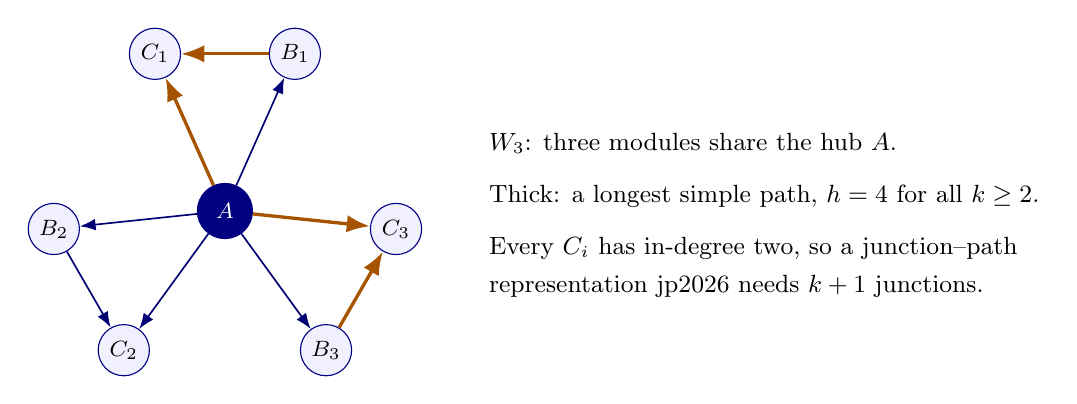
\begin{tikzpicture}[>=Latex,scale=0.95,
  sp/.style={circle,draw=blue!50!black,fill=blue!6,minimum size=6.5mm,inner sep=0pt,font=\footnotesize},
  hub/.style={circle,draw=blue!50!black,fill=blue!50!black,text=white,minimum size=7mm,inner sep=0pt,font=\footnotesize},
  ar/.style={->,semithick,blue!45!black}, hl/.style={->,very thick,orange!65!black}]
\node[hub] (A) at (0,0) {$A$};
\foreach \i/\ang in {1/90,2/210,3/330}{
  \node[sp] (B\i) at (\ang-24:2.3) {$B_{\i}$};
  \node[sp] (C\i) at (\ang+24:2.3) {$C_{\i}$};
}
\draw[ar] (A)--(B2); \draw[ar] (B2)--(C2); \draw[ar] (A)--(C2);
\draw[hl] (A)--(C1); \draw[hl] (B1)--(C1); \draw[ar] (A)--(B1);
\draw[hl] (A)--(C3); \draw[hl] (B3)--(C3); \draw[ar] (A)--(B3);
\node[font=\small,align=left,anchor=west] at (3.4,0.9) {$W_3$: three modules share the hub $A$.};
\node[font=\small,align=left,anchor=west] at (3.4,0.2) {Thick: a longest simple path, $h=4$ for all $k\ge2$.};
\node[font=\small,align=left,anchor=west] at (3.4,-0.5) {Every $C_i$ has in-degree two, so a junction--path};
\node[font=\small,align=left,anchor=west] at (3.4,-1.0) {representation \citep{jp2026} needs $k+1$ junctions.};
\end{tikzpicture}
\caption{The windmill family. Each arrow is a two-channel core \eqref{eq:chemistry}. The number of undirected cycles and the number of shared branching species grow with $k$, while $h$ stays at four.}
\label{fig:windmill}
\end{figure}

On $W_k$ the guarantees at hand compare as follows. Interval elimination on forests does not apply, since every module is an undirected cycle. In a junction--path decomposition \citep{jp2026}, an interior vertex of a path has in-degree and out-degree one among the selected cores, so the hub and every $C_i$ are junctions, and the bound $\mathcal{A}^{O(k+1)}$ of that paper has an exponent that grows with $k$. A decision procedure for the existential theory of the reals that ignores the graph has a guarantee exponential in the number $2k+1$ of variables \citep{basu2014,renegar1992}. Theorems~\ref{thm:main} and~\ref{thm:fpt} give a fixed polynomial in $k$ and $B$, for \emph{all} rational factors and boxes on these graphs, including incompatible and zero-margin instances. These are comparisons of proved upper bounds. Windmills have a simple block structure, and nothing here shows that other methods are slow on them.

\begin{remark}[Generic nested elimination]\label{rem:nested}
Proposition~\ref{prop:graphs}(b) also suggests the generic alternative: eliminate the variables one at a time from the leaves of a depth-first forest by real quantifier elimination, with the at most $h$ ancestor variables free. This runs in polynomial time for every fixed $h$, so polynomiality on fixed-$h$ classes is within the reach of general tools. But the messages are semialgebraic sets in up to $h$ variables, each level raises the number of polynomials to a power of order $2(h+1)$, and a routine estimate gives an exponent of $n$ of order $(2h+2)^{h+1}$; we have not tried to optimize this estimate, which is an upper bound on one strategy. Algorithm~3 is the same elimination order carried out inside the class of monotone two-variable constraints, which is what keeps the exponent of $n$ fixed.
\end{remark}

\begin{proof}[Proof of Proposition~\ref{prop:barrier}]
Let $G_P$ and $F_P$ be the compositions of the lower and upper responses along the path. If $z$ is productive then $z_0=x_0$ and, by induction with Lemma~\ref{lem:edge} and monotonicity, $G_P(x_0)<z_m<F_P(x_0)$; with $z_m\ge\lambda$ this gives $F_P(x_0)>\lambda$. Conversely let $F_P(x_0)>\lambda$ and choose $y\ge\lambda$ with $G_P(x_0)<y<F_P(x_0)$, which is possible because $G_P<F_P$ on $(0,1)$. For $\theta\in[0,1]$ let $z_0=x_0$ and $z_i=(1-\theta)G_i(z_{i-1})+\theta F_i(z_{i-1})$. The endpoint $z_m$ depends continuously on $\theta$ and runs from $G_P(x_0)$ to $F_P(x_0)$, so $z_m=y$ for some $\theta\in(0,1)$, and then every core is productive by \eqref{eq:gap}. Activities decrease along the path, so $z_i\in[y,x_0]\subseteq[\lambda,1]$. Each $F_i$ squares the denominator of its argument, which gives the bit length.
\end{proof}

\section{Consequences of the order structure}\label{sec:consequences}

\subsection{Least required inventory}
\begin{corollary}\label{cor:inventory}
Let $t\ge0$ and $\St\neq\varnothing$. The state $z_*(t)$ returned by Algorithm~1 or Algorithm~3 minimizes every coordinatewise nondecreasing function $C\colon\R^V\to\R$ over $\St$; in particular it minimizes every weighted inventory $\sum_vw_vz_v$ with $w_v\ge0$.
\end{corollary}
\begin{proof}
$z_*(t)\le z$ coordinatewise for every $z\in\St$.
\end{proof}
The statement concerns a fixed weak margin. The set of productive states is not closed and in general has no least element, and the rational witness of Lemma~\ref{lem:round} spends part of the margin. Inventory here means activities of the internal species; nothing is asserted about food consumption or enzyme cost.

\subsection{Capacity}
For $E\neq\varnothing$ define the \emph{capacity}
\[
  \delta_*=\max_{z\in\prod_v[\ell_v,u_v]}\ \min_{e\colon u\to v}\ \min\bigl\{z_v-G_e(z_u),\ F_e(z_u)-z_v\bigr\},
\]
which exists by compactness and may be negative. Then $\St\neq\varnothing$ if and only if $t\le\delta_*$, and a productive state exists if and only if $\delta_*>0$.

\begin{proposition}[Capacity scale]\label{prop:capacity}
With $\rho_e=a_e/b_e$ and $\kappa(\rho)=\rho/\bigl(8(\rho+1)(\rho+2)\bigr)$,
\begin{equation}\label{eq:capacity}
  \delta_*\ \le\ \min_{e\colon u\to v}\ \kappa(\rho_e)\max_{x\in[\ell_u,u_u]}4x(1-x)\ \le\ \min_e\kappa(\rho_e)\ \le\ \kappa(\sqrt2)=\frac{3-2\sqrt2}{8}\approx0.02145 .
\end{equation}
For a single core whose boxes contain $x=\tfrac12$ and $y=\tfrac12\bigl(G(\tfrac12)+F(\tfrac12)\bigr)$, one has $\delta_*=\kappa(\rho)$ exactly; for unit factors $\delta_*=\tfrac1{48}$, attained at $(\tfrac12,\tfrac{17}{48})$.
\end{proposition}
\begin{proof}
The smaller of two numbers is at most half their sum, and the sum of the two normalized residuals of $e$ is $F_e(z_u)-G_e(z_u)$, given by \eqref{eq:gap}. Since $\rho/((\rho+1)(\rho+2))=1/(\rho+3+2/\rho)$ and $\rho+2/\rho\ge2\sqrt2$, the maximum of $\kappa$ is at $\rho=\sqrt2$; equivalently $(3-2\sqrt2)(a+b)(a+2b)-ab=(3-2\sqrt2)(a-\sqrt2\,b)^2$. For one core, choosing $y$ at the midpoint of the band equalizes the two residuals at half the band width, and $x=\tfrac12$ maximizes the width.
\end{proof}

The two inequalities are compiled as \lean{min_residual_le_capacity} and \lean{ratio_factor_le}. The universal ceiling is approached but not attained by rational ratios. The root equation $x(1-x)=12t$ of Example~\ref{ex:unitedge} is the capacity computation for the unit core: its discriminant $1-48t$ vanishes at $\delta_*=\tfrac1{48}$. Because $\St\ne\varnothing$ is decided for any rational $t\ge0$ by Algorithm~1 with the local tests of Lemma~\ref{lem:bits}(c), bisection in $t$ brackets $\delta_*$ to any prescribed dyadic accuracy and returns a rational state whose margin is within that accuracy of optimal. Computing $\delta_*$ exactly, as an algebraic number, would require a decomposition of the margin axis at all critical values and is not done here.

\subsection{Interval uncertainty in the ratios}
\begin{proposition}[Robust compatibility]\label{prop:robust}
Let each ratio range independently over $[r_e^-,r_e^+]\subset(0,\infty)$. A state $x\in(0,1]^V$ is productive for \emph{all} realizations of the ratios if and only if
\begin{equation}\label{eq:robust}
   G_{r_e^+}(x_u)<x_v<F_{r_e^-}(x_u)\qquad\text{for every } e\colon u\to v,
\end{equation}
where the subscript denotes the ratio. The width of this band is
\begin{equation}\label{eq:robustwidth}
   F_{r^-}(x)-G_{r^+}(x)=\frac{(2r^--r^+)\,x(1-x)}{(r^-+1)(r^++2)} ,
\end{equation}
so an edge with $r_e^+\ge2r_e^-$ makes robust compatibility impossible, and this threshold is sharp for a single core. For rational $r_e^\pm$, Theorems~\ref{thm:main} and~\ref{thm:fpt} hold for the system \eqref{eq:robust} with the same bounds.
\end{proposition}
\begin{proof}
On $[0,1]$ both responses are nondecreasing in the ratio: $\partial_rF_r=x(1-x)/(r+1)^2$ and $\partial_rG_r=2x(1-x)/(r+2)^2$. So the intersection of the bands over $r\in[r^-,r^+]$ is \eqref{eq:robust}, and \eqref{eq:robustwidth} is a direct computation. Sections~\ref{sec:model}--\ref{sec:fpt} use, for each edge, only one increasing quadratic forward map of the form $G_r+t$ and one reverse map of the form $F_{r'}^{-1}(\cdot+t)$ with their analyticity, positivity at zero and derivative bounds; they never use that $r=r'$.
\end{proof}

The monotonicity in the ratio and the obstruction are compiled as \lean{lower_mono_ratio}, \lean{upper_mono_ratio} and \lean{robust_band_empty}. The quantifier order is $\exists x\,\forall r$: one state for all realizations, which is stronger than compatibility of every realization separately. Independent factor boxes $a_e\in[a_e^-,a_e^+]$, $b_e\in[b_e^-,b_e^+]$ give $r_e^-=a_e^-/b_e^+$ and $r_e^+=a_e^+/b_e^-$ for positivity; guaranteed \emph{magnitudes} of the residuals depend on the factors and not only on their ratio, and are treated at a fixed state in Section~\ref{sec:example}.

\begin{remark}[Weighted demands]\label{rem:weights}
Replace the two margins of edge $e$ in \eqref{eq:margin} by $t\,\omega_e^-$ and $t\,\omega_e^+$ with positive rational weights. The implication maps become $G_e+t\omega_e^-$ and $F_e^{-1}(\cdot+t\omega_e^+)$ and keep every property used above, so both algorithms and their bounds carry over with the weights included in $B$; in Lemma~\ref{lem:round} one takes $1/N\le t\min_e\min(\omega^-_e,\omega^+_e)/4$. The choice $\omega_e^-=w_{e,u}/(a_e+2b_e)$ and $\omega_e^+=w_{e,v}/(a_e+b_e)$ expresses production demands $R_{e,u}\ge t\,w_{e,u}$ and $R_{e,v}\ge t\,w_{e,v}$ in the original flux units. Zero weights are not covered: they reintroduce identity cycles at positive $t$.
\end{remark}

\section{A certified module and an all-size family}\label{sec:example}

\subsection{The nominal certificate}
Consider the shortcut triangle $A\to B$, $B\to C$, $A\to C$ with factors $(a,b)=(2,1)$, $(2,1)$ and $(1,1)$, which is incompatible when all factors are equal to one (Section~\ref{sec:model}), and the rational state
\begin{equation}\label{eq:state}
  (x_A,x_B,x_C)=\Bigl(\tfrac1{10},\ \tfrac{13}{200},\ \tfrac{43}{1000}\Bigr).
\end{equation}
Table~\ref{tab:triangle} lists the exact currents and residuals. All six residuals are positive; the smallest normalized residual is $\tfrac{209}{120000}$, on the target of $BC$. This is a certificate of compatibility, not an optimizer.

\begin{table}[!ht]
\centering\small
\renewcommand{\arraystretch}{1.25}
\begin{tabular}{@{}lcccccc@{}}
\toprule
Core & $p_e$ & $q_e$ & $R_{e,u}$ & $R_{e,v}$ & $\min R_{e,u}$ on the box & $\min R_{e,v}$ on the box\\
\midrule
$AB$ & $7/100$ & $11/200$ & $1/25$ & $3/200$ & $30351981/10^{9}$ & $16488021/(2\cdot10^{9})$\\
$BC$ & $11/250$ & $1551/40000$ & $671/20000$ & $209/40000$ & $26837781/10^{9}$ & $1175221/(2\cdot10^{9})$\\
$AC$ & $57/1000$ & $33/1000$ & $9/1000$ & $3/125$ & $2411981/10^{9}$ & $38368021/(2\cdot10^{9})$\\
\bottomrule
\end{tabular}
\caption{Exact currents and residuals of the module at the state \eqref{eq:state}, and the exact minima of the residuals over the uncertainty box of Section~\ref{sec:box}: every activity within $\pm10^{-4}$ and every factor within $\pm5\%$.}
\label{tab:triangle}
\end{table}

\subsection{Tolerances}\label{sec:box}
\emph{Factors.} Let every factor vary independently by a relative amount at most $r$ at the fixed state \eqref{eq:state}. Since $p_e,q_e>0$, the worst cases are $R_{e,u}-r(2q_e+p_e)$ and $R_{e,v}-r(p_e+q_e)$. All cores stay productive exactly for
\[
   r<\min_e\min\Bigl\{\frac{R_{e,u}}{2q_e+p_e},\frac{R_{e,v}}{p_e+q_e}\Bigr\}=\frac{209}{3311}=\frac{19}{301}\approx6.31\%,
\]
and at $r=\tfrac{19}{301}$ one residual vanishes. At $r=5\%$ the smallest residual is $\tfrac{869}{800000}$.

\emph{Factors and activities.} Let, in addition, every activity vary independently within $\pm\varepsilon$, with $\varepsilon=10^{-4}$ and $r=5\%$. On these boxes $x-y>0$ and $y-x^2>0$ for every core, $R_{e,u}$ decreases in $x$ and in $a$ and increases in $y$ and in $b$, and $R_{e,v}$ does the opposite. The minima over the whole box are therefore attained at the corners
\begin{align*}
 \min R_{e,u}&=2b(1-r)\bigl[y-\varepsilon-(x+\varepsilon)^2\bigr]-a(1+r)\bigl[x-y+2\varepsilon\bigr],\\
 \min R_{e,v}&=a(1-r)\bigl[x-y-2\varepsilon\bigr]-b(1+r)\bigl[y+\varepsilon-(x-\varepsilon)^2\bigr],
\end{align*}
listed in the last two columns of Table~\ref{tab:triangle}. Every state and every factor assignment in the box is productive, with residuals at least $\tfrac{1175221}{2\cdot10^{9}}\approx5.876\times10^{-4}$. This is a statement about the continuum, proved by monotonicity; no sampling is involved.

\subsection{Replication, food and scaling}\label{sec:windmill}
In the windmill $W_k$ of Proposition~\ref{prop:graphs}, give every module the factors above and the activities \eqref{eq:state}, with the hub shared. Every core sees the same pair of endpoint activities as in the triangle, so the certificate and both tolerance statements hold for every $k\ge1$, on a family with $h=4$. Food is consumed by the second channel only, at rate $q_e$ per core, so a module consumes
\[
  q_{AB}+q_{BC}+q_{AC}=\tfrac{5071}{40000}\approx0.1268
\]
and contributes $R_{AB,A}+R_{AC,A}=\tfrac{49}{1000}$ to the net production of the hub. By the identity $R_{e,u}+R_{e,v}=q_e$ of Lemma~\ref{lem:edge}, total production of internal species equals total food consumption, $k\cdot\tfrac{5071}{40000}$. Dividing all factors by $k$ leaves the state compatible and keeps the aggregate food demand constant, but divides every individual residual by $k$. A polynomial-time certificate does not remove the linear resource cost of a growing assembly.

\subsection{Units and scope of the physical model}\label{sec:units}
A dimensional reading takes ideal activities $x_i=c_i/c_{\mathrm{ref}}$, food concentration $c_F=c_{\mathrm{ref}}$, and a flux scale $J_{\mathrm{ref}}$. The first channel then has forward and reverse first-order constants $J_{\mathrm{ref}}a/c_{\mathrm{ref}}$, the second channel has forward and reverse second-order constants $J_{\mathrm{ref}}b/c_{\mathrm{ref}}^2$, and the dimensional currents are $J_{\mathrm{ref}}$ times \eqref{eq:rates}. All displayed equilibrium constants equal one in these units; the constraints are of the loop-law type of \citet{beard2004}. For mass balance $F$ and all $X_s$ must share elemental composition and charge, for instance as isomers. With $c_{\mathrm{ref}}=1\,\mathrm{mM}$ the state \eqref{eq:state} is $(100,65,43)\,\mu\mathrm{M}$ with uncertainty $\pm0.1\,\mu\mathrm{M}$, and with the illustrative choice $J_{\mathrm{ref}}=1\,\mathrm{mM\,min^{-1}}$ the certified worst residual is $0.5876\,\mu\mathrm{M\,min^{-1}}$. At a productive core $x^2<y<x$, so the affinities $RT\log(x/y)$ and $RT\log(y/x^2)$ and both currents are positive, and the dissipation $p\,RT\log(x/y)+q\,RT\log(y/x^2)$ is positive. The quantity certified here is a \emph{production residual}, which depends on kinetic factors; it differs from the minimal thermodynamic driving force optimized over concentration ranges by \citet{noor2014}, although both are constrained pathway-design problems. These numbers specify a consistent normalized model. They are not measured parameters, and instantaneous productivity of a food-chemostatted network implies neither a steady state nor persistence.

\section{Hypotheses used, and cores of higher order}\label{sec:extensions}

The proofs use the following properties of the constraint system and nothing else about quadratics.
\begin{enumerate}[label=(H\arabic*)]
\item Independent compact boxes, and constraints that are implications $z_j\ge f(z_i)$ with $f$ increasing, so that feasible states dominate all path consequences, the feasible set is min-closed, and a variable can be eliminated exactly (Lemma~\ref{lem:eliminate}).
\item Compositions along walks that are real analytic near the compact seed intervals, so that non-identity cycle maps have finitely many fixed points and distinct walk maps cross finitely often. Any other source of this finiteness would serve equally.
\item At positive margin, no identity cycles; here because every implication map is positive at $0$.
\item Transports whose graphs are described by polynomial equations and sign conditions of bounded degree with a \emph{unique} admissible branch.
\item A number of free seeds per comparison that is bounded (Theorem~\ref{thm:main}) or bounded in terms of $h$ (Theorem~\ref{thm:fpt}).
\item An explicit Lipschitz bound for the responses on the boxes, for the rational output.
\end{enumerate}
Monotonicity and analyticity alone give termination of Algorithm~1 and correctness of Algorithm~3 over the reals, but no effective algebraic execution and no bit bound; conversely degree two is not essential. Rational rate laws of Michaelis--Menten type are \emph{not} covered automatically: poles, range restrictions, non-unique inverse branches and couplings between more than two species have to be examined case by case. Constraints in three or more variables are in general not min-closed.

\begin{theorem}[Cores of fixed order]\label{thm:degree}
Fix an integer $d\ge2$ and replace the second channel of every core by $X_v+(d-1)F\rev dX_u$, so that $q_e=b_e(x_v-x_u^d)$, $R_{e,u}=dq_e-p_e$ and $R_{e,v}=p_e-q_e$. Productivity of a core is equivalent to $G_d(x_u)<x_v<F_d(x_u)$ with
\[
   G_d(x)=\frac{ax+db\,x^d}{a+db},\qquad F_d(x)=\frac{ax+b\,x^d}{a+b},\qquad F_d(x)-G_d(x)=\frac{(d-1)ab\,x\,(1-x^{d-1})}{(a+b)(a+db)},
\]
and Theorems~\ref{thm:main} and~\ref{thm:fpt} hold with constants $C_d,c_d$ and a function $f_d$ depending on $d$.
\end{theorem}
\begin{proof}
The band is a rearrangement, compiled as \lean{order_d_band}. Both responses vanish at $0$, fix $1$, and have derivative at least $a/(a+db)>0$ on $[0,\infty)$, so they are increasing bijections of $[0,\infty)$ with analytic inverses near every nonnegative point, by the analytic inverse function theorem \citep{krantz2002}; this gives (H1)--(H3). The graph of a step is $(a+db)y-ax-dbx^d-(a+db)t=0$, respectively $ay+by^d-(a+b)(x+t)=0$, with $x,y\ge0$ and a unique admissible $y$, which is (H4); (H5) is unchanged. In Lemma~\ref{lem:bits}, (QE) is applied with degree $d$ instead of $2$, which changes $Q$ to $(k+1)^{C_dk}$, and $s_h$ in Lemma~\ref{lem:pieces} depends on $d$. On $[0,1]$ one has $G_d'\le d$ and $F_d'\le d$, so in Lemma~\ref{lem:round} downward rounding with $1/N\le t/(2d)$ keeps the margin $t/2$, which is (H6).
\end{proof}

If $d$ is part of the input, a separate analysis of degree and encoding is required. A single elementary step of molecularity $d$ is chemically unrealistic for large $d$; the theorem is stated to show that the mechanism is not tied to quadratics, and replacing the channel by a chain of bimolecular intermediates would require its own source-equivalence argument.

\section{Formal verification}\label{sec:formal}

The Lean~4 development accompanying the paper compiles against Mathlib in a frozen environment (Lean \lean{v4.30.0}, pinned Mathlib manifest), with warnings promoted to errors; it contains no \lean{sorry}, no added axiom and no \lean{native_decide}, and the reported axioms of the root declarations are \lean{propext}, \lean{Classical.choice} and \lean{Quot.sound}. The sources are in \RepoPhrase, under \lean{proofs/ThermoCoreCompatibility/}. Table~\ref{tab:lean} maps the claims of the paper to declarations in the namespace \lean{ThermoCoreCompatibility.GeneralCompatibility}, except where another module is named.

\begin{table}[!ht]
\centering\footnotesize
\begin{tabular}{@{}>{\raggedright\arraybackslash}p{0.25\linewidth}>{\raggedright\arraybackslash}p{0.40\linewidth}>{\raggedright\arraybackslash}p{0.29\linewidth}@{}}
\toprule
Claim in the paper & Compiled declarations & Conventional part\\
\midrule
Lemma~\ref{lem:edge}: band, residual identities & \lean{MultiInterface.WeightedPair}: \lean{productive_iff}, \lean{residual_lower}, \lean{residual_upper}, \lean{gap}; \lean{RobustExample.residual_sum} & none\\
Implications \eqref{eq:maps}, explicit inverse & \lean{inverseUpper}, \lean{upper_inverseUpper}, \lean{inverseUpper_le_iff}, \lean{inverseUpper_monotoneOn}, \lean{continuous_inverseUpper}, \lean{boxed_margin_iff_implications} & analyticity of compositions\\
Lemma~\ref{lem:least}: least state, tight support & \lean{compact_min_closed_has_least}, \lean{margin_min}, \lean{margin_isClosed}, \lean{margin_has_least}, \lean{active_support_coverage} & none\\
Lemma~\ref{lem:jump}: forced root & \lean{lifted_cycle_violation}, \lean{fixed_between_violation_and_prefixed}, \lean{least_cycle_root_preserves_bound}, \lean{no_cycle_root_rejects_prefixed} & extraction of the cycle from the label path (Lemma~\ref{lem:rounds})\\
Lemmas~\ref{lem:termination}, \ref{lem:fibres}: finiteness & \lean{finite_cycle_roots_of_violation}, \lean{finite_cycle_roots}, \lean{consumed_tokens_injective}, \lean{cycle_jump_count_bound}, \lean{no_infinite_anchor_updates} & identification of tokens with graph cycles\\
Remark~\ref{rem:failures}(a) & \lean{Interaction}: \lean{support_least}, \lean{full_least}, \lean{selected_support_is_tight_at_global}, \lean{selected_least_not_global} & six-species instance (exact computation)\\
Theorem~\ref{thm:trace}, Corollary~\ref{cor:uniform} & \lean{feasible_of_candidate_transport}, \lean{boxed_strict_iff_source}, \lean{strict_iff_positive_margin}, \lean{margin_downward}, \lean{strict_decision_of_stable_margin}, \lean{source_decision_at_stable_threshold}, \lean{no_productive_source_of_no_threshold_state} & Lemmas~\ref{lem:projection}, \ref{lem:branches}: elimination, CAD, branches; the stability hypothesis\\
Lemma~\ref{lem:round} & \lean{round_down_margin}; \lean{BeyondJunction.MarginTransfer} & bisection, output size\\
Lemma~\ref{lem:eliminate}, Proposition~\ref{prop:elimcorrect} & \lean{IsNextMap}, \lean{IsNextMap.mono}, \lean{IsNextMap.fixed_of_mem}, \lean{eliminate_vertex_iff}, \lean{eliminated_value_least}, \lean{generated_map_mono} & closedness of $U_w$, induction over the forest\\
Corollary~\ref{cor:inventory} & \lean{least_minimizes_monotone}, \lean{least_minimizes_inventory} & none\\
Proposition~\ref{prop:capacity} & \lean{min_residual_le_capacity}, \lean{ratio_factor_le} & attainment for one core\\
Proposition~\ref{prop:robust} & \lean{lower_mono_ratio}, \lean{upper_mono_ratio}, \lean{robust_band_empty} & reduction of the algorithms\\
Section~\ref{sec:example} & \lean{triangle_nominal}, \lean{triangle_box_corners_positive} & monotonicity reduction to corners\\
Theorem~\ref{thm:degree} & \lean{order_d_band} & analytic and algebraic part\\
Theorems~\ref{thm:main}, \ref{thm:fpt}: bit bounds; Lemma~\ref{lem:pieces}; Section~\ref{sec:parameter} & none & entirely conventional\\
\bottomrule
\end{tabular}
\caption{Claim-to-proof concordance. ``Compiled'' means that a strict compilation receipt exists for the current source hash of the module.}
\label{tab:lean}
\end{table}

The two root declarations state, for arbitrary finite index types, real factors and boxes, that if weak feasibility at margin $\sigma$ is equivalent to weak feasibility at margin $t$ for all $0<\sigma\le t$, then the existence of a boxed state at which every core is productive, in the literal sense of the source predicate \lean{Productive}, is equivalent to the existence of a boxed state of margin $t$; and that the absence of the latter excludes the former. The stability hypothesis is what Theorem~\ref{thm:trace} provides for $t=t_1$, and Corollary~\ref{cor:uniform} for $t=t_0$, by conventional real-algebraic arguments. The elimination lemma is compiled for arbitrary index types, an arbitrary set $U$ with a next-map, and arbitrary monotone outgoing maps; it uses no continuity and no algebra. The declarations do not construct decompositions, do not traverse graphs and do not establish any complexity statement, and the development is not an end-to-end verified decision procedure. A small rational witness checker accompanies the sources; it verifies supplied witnesses only.

\section{Discussion and open questions}\label{sec:discussion}

The structural content of the paper is twofold. First, a finite representation theorem: the least state of a system of monotone, analytic, two-variable implications with unique algebraic branches is assembled from box endpoints and roots of \emph{fixed} simple-cycle equations, each transported along one simple path, uniformly for small positive margins. Second, a closure property: such systems are closed under exact elimination of a variable, the disconnected projections being recorded by next-maps, and along a forest of bounded depth the description grows additively. The algorithms are stated for the two-reaction cores of \citep{kosc2025,tcch2026,jp2026}, where they turn a problem that was decided only for forests and for boundedly many junctions into one that is fixed-parameter tractable in the longest path on all graphs.

\begin{question}
Is there an algorithm with cost $2^{\poly(h)}\poly(n,B)$? Theorem~\ref{thm:fpt} has an iterated exponential $f$, caused by walks of length $2^{h+1}$, while Theorem~\ref{thm:main} has $(h+2)^{O(h)}$ arithmetic but the factor $J$.
\end{question}

\begin{question}
Is the number $J$ of jumps of Algorithm~1 bounded by $\varphi(h)\poly(n)$ on all graphs, for a suitable rule for choosing the detected cycle? The token bound counts all roots of all simple cycles, which is $n^{\Theta(q)}$ on $K_{q,n}$. There, eliminating the $n$ leaves by Lemma~\ref{lem:eliminate} leaves a system on $q$ hubs whose maps are envelopes with near-linearly many pieces, and a jump to a fixed point of the \emph{attaining piece} either lands on a fixed point of the envelope cycle map or leaves the piece for good, which bounds the jumps by $\varphi(q)\,n^{1+o(1)}$; we do not know a rule that achieves this on general graphs without computing envelopes.
\end{question}

\begin{question}
Can the sign of $F_m\circ\dots\circ F_1(x_0)-\lambda$ in Proposition~\ref{prop:barrier} be decided in time polynomial in $m$ and $B$? A positive answer is necessary for a polynomial-time algorithm on all graphs; a hardness result for this special sign problem would be of independent interest.
\end{question}

\begin{question}
Can the capacity $\delta_*$ be computed exactly, as an algebraic number with a certified optimizer, within the bounds of Theorems~\ref{thm:main} or~\ref{thm:fpt}? This asks for the critical margins at which branches of Lemma~\ref{lem:branches} are born, merge or exchange test results, as in Figure~\ref{fig:cycle}(c).
\end{question}

\begin{question}
Which reversible mass-action motifs beyond \eqref{eq:chemistry} and Theorem~\ref{thm:degree} satisfy (H1)--(H6)? Cores with three or more internal species give constraints in more than two variables, for which min-closure can fail.
\end{question}

Practical matters are also open. A complete implementation needs certified interval filters for the overwhelming majority of sign decisions and the projected exact fallback of Lemma~\ref{lem:bits} for the rest; in an exploratory prototype of cycle acceleration, exact comparison of nested radicals, not the number of jumps, was the bottleneck, which is the difficulty that bounded ancestry and retained seeds are designed to remove. Treating the margin as an infinitesimal, rather than fixing an a priori threshold, keeps the working precision tied to the comparisons actually made. No runtime claim is made.

\appendix
\section{Reproducibility}\label{app:repro}

The source package contains \lean{main.tex}, \lean{refs.bib}, the figure script \lean{make_figures.py}, the numerical sanity check \lean{sanity_elimination.py} described in Section~\ref{sec:fpt}, and \lean{check_paper.py}, which replays with exact rational and symbolic arithmetic every number and identity printed in the paper: the identities of Lemma~\ref{lem:edge} and the explicit inverse; Example~\ref{ex:unitedge}, including $\alpha=(5-\sqrt{13})/10$ and the tight least state; the three examples of Remark~\ref{rem:failures}; the longest paths of stars, complete graphs and windmills and the inequality $m\le hn$ on them; an instance of Proposition~\ref{prop:barrier} with its bit growth; Proposition~\ref{prop:capacity}, including the maximizer $\rho=\sqrt2$ and the unit optimum; the identities of Proposition~\ref{prop:robust}; Table~\ref{tab:triangle}, the radius $\tfrac{19}{301}$, the value $\tfrac{869}{800000}$, the food and hub totals; and the identities and derivative bounds of Theorem~\ref{thm:degree} for $d=2,\dots,6$. It requires Python with SymPy and ends with the line \lean{"status": "PASS"}. The script is a certificate replay and not an implementation of the algorithms. The core of the certificate for Section~\ref{sec:example} is short enough to state:

\begin{verbatim}
from fractions import Fraction as Q
edges = [('AB', Q(1,10),   Q(13,200),  Q(2), Q(1)),
         ('BC', Q(13,200), Q(43,1000), Q(2), Q(1)),
         ('AC', Q(1,10),   Q(43,1000), Q(1), Q(1))]
r, eps = Q(1,20), Q(1,10000)
radii, worst, food = [], [], Q(0)
for name, x, y, a, b in edges:
    p, q = a*(x-y), b*(y-x*x)
    ru, rv = 2*q-p, p-q
    assert ru > 0 and rv > 0
    radii += [ru/(2*q+p), rv/(p+q)]
    assert x-eps > y+eps and y-eps > (x+eps)**2
    worst += [2*b*(1-r)*(y-eps-(x+eps)**2) - a*(1+r)*(x-y+2*eps),
              a*(1-r)*(x-y-2*eps) - b*(1+r)*(y+eps-(x-eps)**2)]
    food += q
assert min(radii) == Q(19,301) and food == Q(5071,40000)
assert min(worst) == Q(1175221,2000000000) > 0
\end{verbatim}

The Lean modules named in Table~\ref{tab:lean} are in the subdirectories \lean{GeneralCompatibility}, \lean{BeyondJunction} and \lean{MultiInterface} of \lean{proofs/ThermoCoreCompatibility/}, together with their strict compilation receipts; the archive \lean{lean_sources.zip} of the source package contains them with the toolchain pin and a short guide.

\bibliographystyle{abbrvnat}
\bibliography{refs}

\end{document}
